\documentclass[lettersize,journal]{IEEEtran}
\usepackage{amsmath,amsfonts}
\usepackage{algorithmic}
\usepackage{algorithm}
\usepackage{array}
\usepackage[caption=false,font=normalsize,labelfont=sf,textfont=sf]{subfig}
\usepackage{textcomp}
\usepackage{stfloats}
\usepackage{url}
\usepackage{verbatim}
\usepackage{graphicx}
\usepackage{cite}
\usepackage{booktabs}
\usepackage[table]{xcolor}
\usepackage[hidelinks]{hyperref}
\hyphenation{op-tical net-works semi-conduc-tor IEEE-Xplore}

\begin{document}

\title{Geometry-Guided Feed-Forward Regression for LiDAR-Inertial-Camera Photo-Realistic 2DGS Mapping}
% 作者与单位信息按 IEEE 期刊模板的 \thanks 方式填写，保留模板原有排版风格。
\author{Puwei Zhao$^{\dagger}$, Yiduo Zhou$^{\dagger}$, Yiming Fan$^{\dagger}$, Kun Qian$^{*}$,~\IEEEmembership{Member,~IEEE}, and Tong Shi%
\thanks{$\dagger$ Puwei Zhao, Yiduo Zhou, and Yiming Fan contributed equally to this work.}%
\thanks{$*$ Corresponding author: Kun Qian.}
\thanks{Puwei Zhao, Yiduo Zhou, Yiming Fan, Kun Qian and Tong Shi are with the School of Automation, Southeast University, Nanjing, China (e-mail: kqian@seu.edu.cn).}%
\thanks{This work is sponsored by Guangdong Basic and Applied Basic Research Foundation (No. 2025A1515010397), the Taihu Lake Innovation Fund for the School of Future Technology of Southeast University, and the 2025 Jiangsu College Students' Innovation and Entrepreneurship Training Program (NO. S202510286238)}}
\maketitle

\begin{abstract}
Incremental 3D scene reconstruction requires a system to continuously extend the map while ingesting new observations frame by frame, and the limited online optimization budget makes the initial quality of newly inserted Gaussians a decisive factor for the accumulated map quality. Existing incremental mapping systems based on 3D Gaussian Splatting still suffer from two coupled limitations in representation and initialization: 3D ellipsoidal primitives lack explicit surface-normal semantics, and rule-based initialization strategies cannot fully exploit external geometric priors. To address these issues jointly, we propose a context-aware feedforward Gaussian regression system for incremental 2DGS scene reconstruction. The system uses 2DGS surfels as the map's base representation and fuses SPNet depth completion with monocular normal priors to construct candidate points and their geometric directions. A feedforward regression network aggregates image-rendering context from the current frame and historical frames via cross-attention and anchors surfel rotations to the normal prior through Gram-Schmidt orthogonalization, directly predicting complete surfel attributes in a single forward pass. Training is completed through a self-distillation loop and requires no externally labeled dataset. Experiments on R3LIVE, MCD, and our self-collected dataset in Southeast University campuse show that the proposed method outperforms existing baselines across diverse test scenes, with an average improvement of 1.28 dB PSNR over the closest multisensor incremental Gaussian mapping baseline on R3LIVE. Ablation studies further verify that the feedforward regressor consistently improves the early convergence quality of newly inserted Gaussians under a limited optimization budget.
\end{abstract}

\begin{IEEEkeywords}
Incremental reconstruction, 2D Gaussian Splatting, LiDAR-inertial-camera fusion, feedforward regression, self-distillation.
\end{IEEEkeywords}

\section{Introduction}
\IEEEPARstart{I}{ncremental} 3D scene reconstruction plays a critical role in time-sensitive field tasks such as autonomous driving, disaster response, industrial inspection, and cultural heritage preservation. These applications require a system to continuously ingest new observations while progressively building a geometrically consistent and photorealistic 3D map. However, the operational constraints of online systems imply that the computation budget available for map optimization at each frame is extremely limited, and newly inserted map elements often need to support subsequent rendering after only a few optimization steps. As a result, the initial quality of newly inserted elements directly affects the accumulated quality of the entire map.

Since NeRF~\cite{mildenhall2021nerf}, radiance-field-based methods have shown strong novel-view rendering capability, while explicit accelerations such as Plenoxels~\cite{fridovich2022plenoxels} and Instant-NGP~\cite{muller2022instant} reduce part of the optimization cost. 3D Gaussian Splatting (3DGS)~\cite{kerbl20233d} further replaces volumetric integration with explicit Gaussian primitives and differentiable rasterization, making high-quality rendering much more practical for online mapping. Recent incremental Gaussian systems, including MonoGS~\cite{matsuki2024gaussian}, GS-SLAM~\cite{yan2024gs}, SplaTAM~\cite{keetha2024splatam}, and Gaussian-LIC2~\cite{lang2025gaussianlic2}, have consequently shown that photorealistic Gaussian maps can be expanded online under monocular, RGB-D, and multisensor settings.

However, two coupled limitations remain in existing incremental Gaussian backends. At the representation level, standard 3DGS~\cite{kerbl20233d} models scenes with 3D ellipsoidal primitives, which weakens geometric consistency in depth rendering and makes it difficult to directly couple external normal priors with the map. Surfel-oriented variants such as 2DGS~\cite{huang20242d}, GaussianSurfels~\cite{dai2024high}, and PGSR~\cite{chen2024pgsr} improve surface fidelity, but they have not been systematically adopted in incremental LiDAR-inertial-camera mapping. At the initialization level, current systems still mostly rely on rule-based insertion; even when learned geometric priors are introduced, they are usually used only to decide where to add Gaussians. For example, Gaussian-LIC2~\cite{lang2025gaussianlic2} uses SPNet~\cite{wang2024scale} to densify sparse LiDAR depth, but does not extend the learned prior to full Gaussian attribute prediction. Meanwhile, feedforward reconstruction models have evolved from pixelNeRF~\cite{yu2021pixelnerf} and MVSNeRF~\cite{chen2021mvsnerf} to Gaussian-native predictors such as pixelSplat~\cite{charatan2024pixelsplat} and MVSplat~\cite{chen2024mvsplat}, showing in offline settings that Gaussian attributes can be regressed directly from image features. In short, if the representation lacks geometric interpretability, rule-based initialization cannot fully exploit external priors; if initialization remains hand-crafted, the benefit of a geometrically interpretable representation cannot be fully realized at insertion time.

To address these issues, we propose a context-aware feedforward Gaussian regression system for incremental 2DGS scene reconstruction. The system uses 2DGS surfels as the map's base representation. Under the condition that an external stable front end provides poses, it fuses depth completion and monocular normal priors to construct initial points and their geometric directions, and then lets a feedforward regression network jointly exploit image and rendering features from the current frame and historical frames to directly predict the complete surfel attributes of newly inserted Gaussians in a single forward pass before handing them to online photometric optimization. The system also includes a complete self-distillation training loop that enables training and deployment of the feedforward network without any external labeled dataset.

The main contributions of this paper are summarized as follows:

\begin{itemize}
    \item A geometry-aware incremental Gaussian mapping backend based on 2DGS surfels. Unlike existing incremental systems that default to 3DGS volumetric Gaussians, we adopt the surfel-based representation of 2DGS and build a unified geometric pipeline around surfel normal semantics by combining SPNet depth completion and the DA3 normal prior. Depth distortion and normal consistency constraints then drive map updates, providing a geometrically interpretable representation foundation for subsequent feedforward Gaussian insertion.

    \item A context-aware feedforward Gaussian insertion method. We propose a feedforward attribute regression method that replaces conventional rule-based initialization. For each candidate point, the method jointly uses raw and rendered image features from the current frame and historical frames, fuses multiview context via point-wise cross-attention, and anchors surfel rotation to the DA3 normal prior through Gram-Schmidt orthogonalization, directly regressing the complete 2DGS surfel attributes in a single forward pass.

    \item A self-distillation training loop for online incremental mapping. We construct a self-distillation pipeline that allows the feedforward insertion method to be trained without any external labeled dataset. The loop organizes training samples around Gaussians, uses Gaussian snapshots at a predefined training-step budget as supervision signals, and synchronously captures point-wise context and geometric priors at that time, enabling a self-boosting process from online mapping to offline training and back to redeployment.
\end{itemize}

\section{Related Works}
This work focuses on how to build a Gaussian map backend that is better suited for incremental scene reconstruction under the condition that an external stable front end provides poses. Related research can therefore be discussed from three directions: photorealistic radiance field reconstruction and Gaussian representations, incremental visual Gaussian reconstruction systems, and multisensor Gaussian reconstruction.

\subsection{Photorealistic Radiance Field Reconstruction and Gaussian Representations}

NeRF~\cite{mildenhall2021nerf} and accelerated radiance-field variants such as Plenoxels~\cite{fridovich2022plenoxels} and Instant-NGP~\cite{muller2022instant} established photorealistic scene reconstruction, but they still depend on volumetric rendering. 3DGS~\cite{kerbl20233d} makes explicit splatting practical for real-time rendering and has therefore become the dominant representation in recent photorealistic mapping systems.

Two follow-up directions are especially relevant to this work. For geometric fidelity, 2DGS~\cite{huang20242d}, GaussianSurfels~\cite{dai2024high}, and PGSR~\cite{chen2024pgsr} improve surface consistency through surfel-oriented or planar constraints. For learned priors, generalizable reconstruction evolved from pixelNeRF~\cite{yu2021pixelnerf} and MVSNeRF~\cite{chen2021mvsnerf} to Gaussian feedforward models such as pixelSplat~\cite{charatan2024pixelsplat} and MVSplat~\cite{chen2024mvsplat}. These two lines together suggest that an incremental Gaussian backend should ideally combine a geometrically interpretable primitive with learned attribute prediction.

\subsection{Incremental Visual Gaussian Reconstruction Systems}

MonoGS~\cite{matsuki2024gaussian} first showed that 3DGS can serve as a unified map for monocular online SLAM. GS-SLAM~\cite{yan2024gs} and SplaTAM~\cite{keetha2024splatam} further demonstrated efficient Gaussian map expansion and structured RGB-D updates, while Photo-SLAM~\cite{huang2024photo} highlighted the benefit of decoupling pose estimation and photorealistic mapping. These systems establish the feasibility of incremental visual Gaussian reconstruction, but they still inherit 3DGS volumetric primitives and mainly improve performance through tracking or optimization strategy.

From the perspective of this paper, the remaining gap is therefore not whether Gaussian maps can be updated online, but whether the backend representation and insertion mechanism themselves are suitable for geometry-aware incremental reconstruction under a limited online optimization budget.

\subsection{Multisensor Gaussian Reconstruction}

Outdoor and large-scale mapping requires wider coverage and stronger geometric constraints than pure visual systems can reliably provide. Gaussian-LIC~\cite{lang2024gaussian} first combined LiDAR-inertial-camera fusion with real-time 3DGS mapping, using LiDAR points and online triangulated visual points to initialize new Gaussians. GS-LIVM~\cite{xie2024gs} and GS-LIVO~\cite{hong2025gs} further extended multisensor Gaussian mapping toward large-scale reconstruction and resource-constrained deployment.

Gaussian-LIC2~\cite{lang2025gaussianlic2} then moved the field closer to sparse-LiDAR operation by combining sparse LiDAR with SPNet depth completion~\cite{wang2024scale} for denser Gaussian initialization. Nevertheless, these systems remain built on 3DGS maps, so learned priors are still weakly coupled to surface orientation and are not used to predict complete Gaussian attributes. This is exactly the gap targeted by our 2DGS-based feedforward insertion backend.

\section{Method}

\providecommand{\methodlead}[1]{\vspace{0.35em}\noindent\textit{#1}}

\begin{figure*}[!t]
\centering
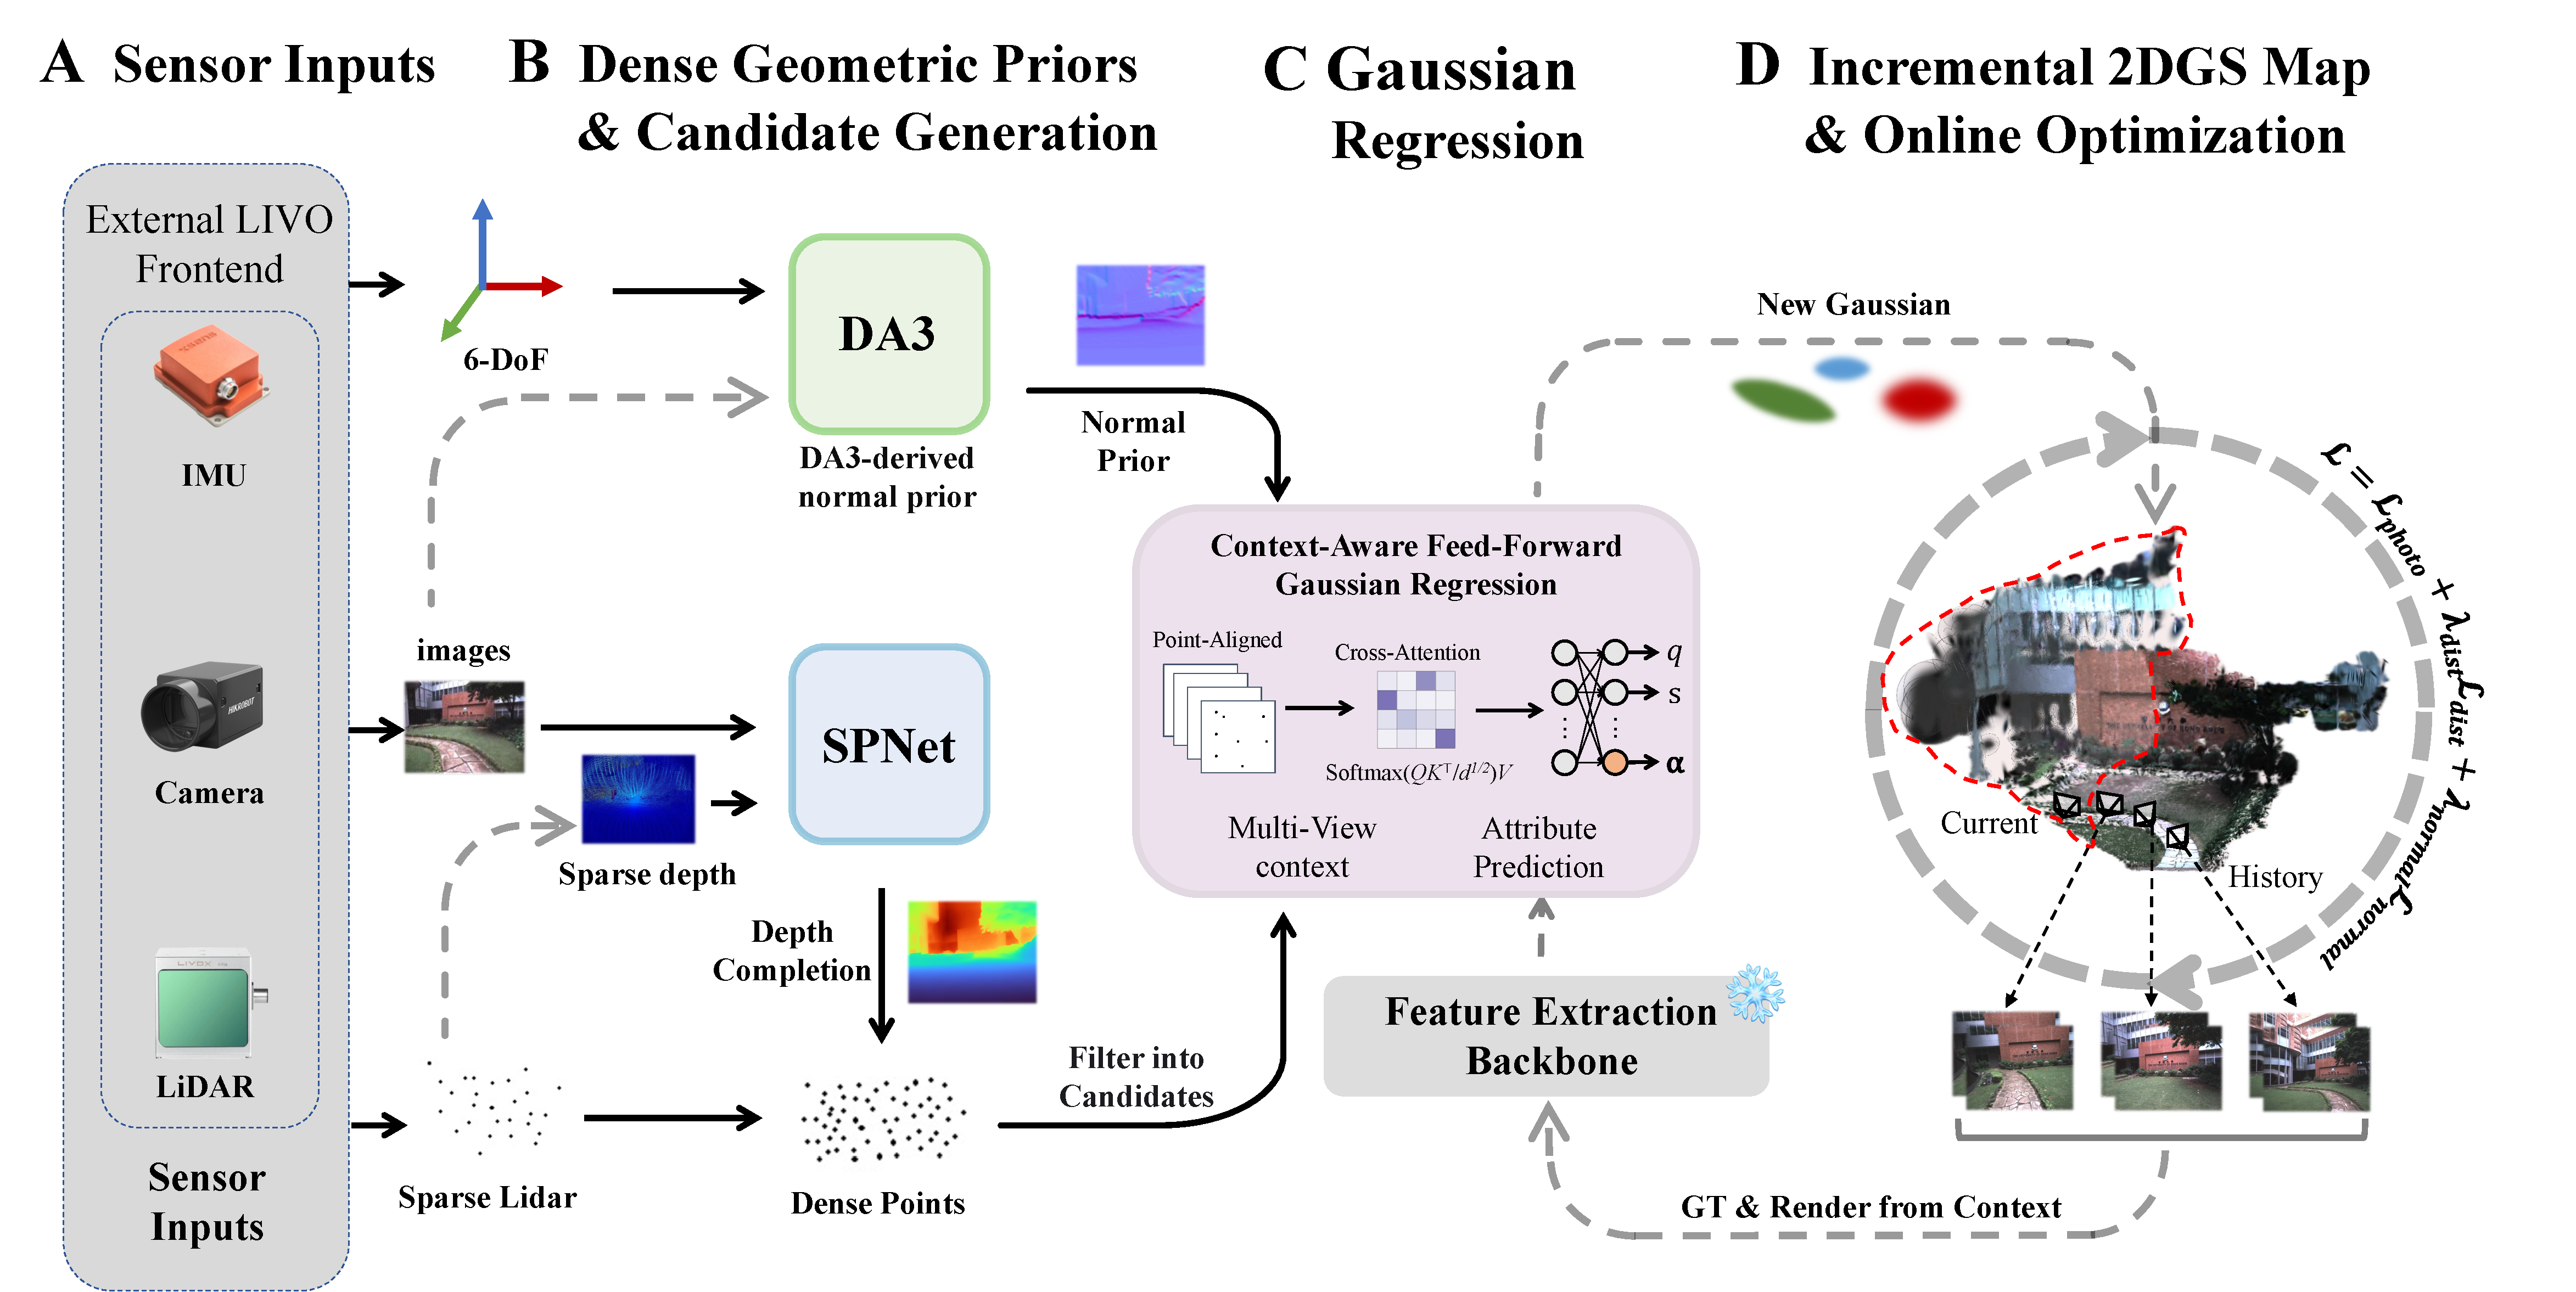
\includegraphics[width=\textwidth,height=0.36\textheight,keepaspectratio]{../../system-pipeline.pdf}
\caption{Overall system pipeline. (A) The external LiDAR-inertial-visual front end provides synchronized RGB images, LiDAR observations, IMU information, and camera poses. (B) The system uses SPNet depth completion and DA3 normal estimation to generate dense geometric priors, which are combined with LiDAR points to form the initial points in under-reconstructed regions. (C) For each candidate point, the feedforward Gaussian regressor aggregates point-aligned multiview context and directly predicts the complete 2DGS surfel attributes. (D) The predicted surfels are inserted into the incremental map and further refined by online optimization, while the current map rendering continues to serve as contextual input for subsequent insertions.}
\label{fig:system_pipeline}
\end{figure*}

\subsection{System Overview}

Our system is an incremental 2DGS scene reconstruction backend built on top of an external pose front end. It receives synchronized data streams in real time from an external LiDAR-Inertial-Camera front end such as R3Live, with each frame containing an RGB image, sparse LiDAR point cloud, and 6-DOF camera pose, and uses 2DGS surfels as the base map representation.

When a new keyframe arrives, the system first projects sparse LiDAR points onto the image plane to form a sparse depth map. After depth completion by SPNet, supplemental initial 3D points are generated in LiDAR blind regions. At the same time, the DA3 monocular depth estimation model predicts dense depth and aligns it with LiDAR, thereby providing normal priors for the initial points. After initial point generation, the system renders the current Gaussian map and identifies under-reconstructed regions according to rendering opacity and color error. Combined with color-gradient filtering and voxel downsampling, it selects the subset of candidate points that truly require new Gaussians. The filtered candidate points and their geometric priors are fed into a feedforward regression network, which uses shared backbone features extracted from the current frame and historical frames, fuses multiview context through cross-attention, and directly regresses the complete surfel attributes of each candidate point in a single forward pass. After the predicted new Gaussians are inserted into the map, the system performs multiple rounds of online optimization on the keyframes inside the sliding window, jointly driving Gaussian attribute convergence with a photometric loss (L1 + SSIM) and 2DGS geometric constraint losses (depth distortion and normal consistency). Non-keyframes only update the pose and do not trigger map expansion.

Training of the feedforward regression network is completed through a self-distillation loop. The system first runs a complete incremental mapping process on the training scenes in \texttt{naive} mode, which does not use the feedforward network and instead relies on conventional rule-based initialization. When the accumulated number of optimization steps for newly added Gaussians in a frame reaches a preset threshold, the system snapshots their current attributes and constructs the corresponding point-wise context and geometric priors at that time as training samples, and then trains the feedforward network offline.

The architecture of the feedforward Gaussian regressor is shown in Fig.~\ref{fig:net_pipeline}.

\subsection{2DGS Representation}

Our system uses 2D Gaussian Splatting (2DGS) as the base map representation. Unlike the 3D ellipsoidal primitives of standard 3DGS, 2DGS compresses Gaussians into two-dimensional oriented Gaussian disks, or surfels, embedded in 3D space, giving each primitive an explicit local planar geometric meaning. Each surfel is defined by a center position $\boldsymbol{\mu} \in \mathbb{R}^3$, two orthogonal tangent directions $\mathbf{t}_u$ and $\mathbf{t}_v$, and corresponding 2D scale factors $(s_u, s_v)$. The normal direction is given by $\mathbf{n} = \mathbf{t}_u \times \mathbf{t}_v$. The orientation is stored as a unit quaternion $\mathbf{q} \in \mathbb{S}^3$, whose corresponding rotation matrix is $\mathbf{R} = [\mathbf{t}_u \mid \mathbf{t}_v \mid \mathbf{n}]$. In addition, each surfel carries opacity $\alpha$ and spherical-harmonic color coefficients to express view-dependent appearance. During rendering, pixel colors are accumulated layer by layer from front to back through alpha blending:

\begin{equation}
\mathbf{c}(\mathbf{x}) = \sum_{i} \mathbf{c}_i \, \alpha_i \, \hat{\mathcal{G}}_i(\mathbf{u}(\mathbf{x})) \prod_{j=1}^{i-1} \left(1 - \alpha_j \, \hat{\mathcal{G}}_j(\mathbf{u}(\mathbf{x}))\right)
\end{equation}

where $\hat{\mathcal{G}}_i$ is the Gaussian weight computed by ray-splat intersection. Depth and normals can be rendered in a similar weighted manner to accumulate geometric information. To fully exploit the surfel-based structure, the system introduces a depth distortion loss $\mathcal{L}_{\text{dist}}$ and a normal consistency loss $\mathcal{L}_{\text{normal}}$ in online optimization, following 2DGS~\cite{huang20242d} and related surfel-based Gaussian reconstruction methods~\cite{dai2024high,chen2024pgsr}.

The core advantage of 2DGS is that each surfel naturally has an explicit normal semantics, which allows external normal priors to be directly coupled with surfel rotation parameters and provides a geometrically interpretable anchor for subsequent feedforward rotation prediction.

\subsection{Dense Geometric Priors}

To generate sufficiently dense and geometrically reasonable initial Gaussian points in incremental mapping, the system jointly uses two complementary modules: SPNet depth completion and DA3 normal guidance.

\methodlead{1) SPNet depth completion:} Sparse LiDAR point clouds cover only a limited portion of the image plane and cannot provide geometric observations for regions outside the LiDAR field of view or for occluded areas. Following the Gaussian-LIC2 pipeline~\cite{lang2025gaussianlic2}, the system uses the SPNet depth completion network~\cite{wang2024scale} to fuse RGB images and sparse LiDAR depth into a dense depth map, and samples supplementary 3D initial points in regions without LiDAR coverage. The SPNet completion points and the original LiDAR projection points are finally merged into the initial point set.

\methodlead{2) DA3 normal guidance:} The system uses DA3~\cite{lin2025da3}, our monocular depth module, to provide an initial normal direction for the surfel corresponding to each initial point. After DA3 infers a relative depth map from the current-frame RGB image, the system aligns it with sparse LiDAR depth via least-squares affine registration to obtain a dense depth map with the correct metric scale, and then computes per-pixel normals by central differencing. Sampling the normal map at the pixel coordinates of each initial point yields the camera-space normal $\mathbf{n}_{\text{cam}} \in \mathbb{R}^3$ for that point.

It should be noted that DA3 normal computation precedes the feedforward regression network: the normal prior is first computed independently by DA3 and then passed to the feedforward network as input, where it is slightly refined and used to construct the full rotation representation, as detailed below.

\begin{figure*}[!t]
\centering
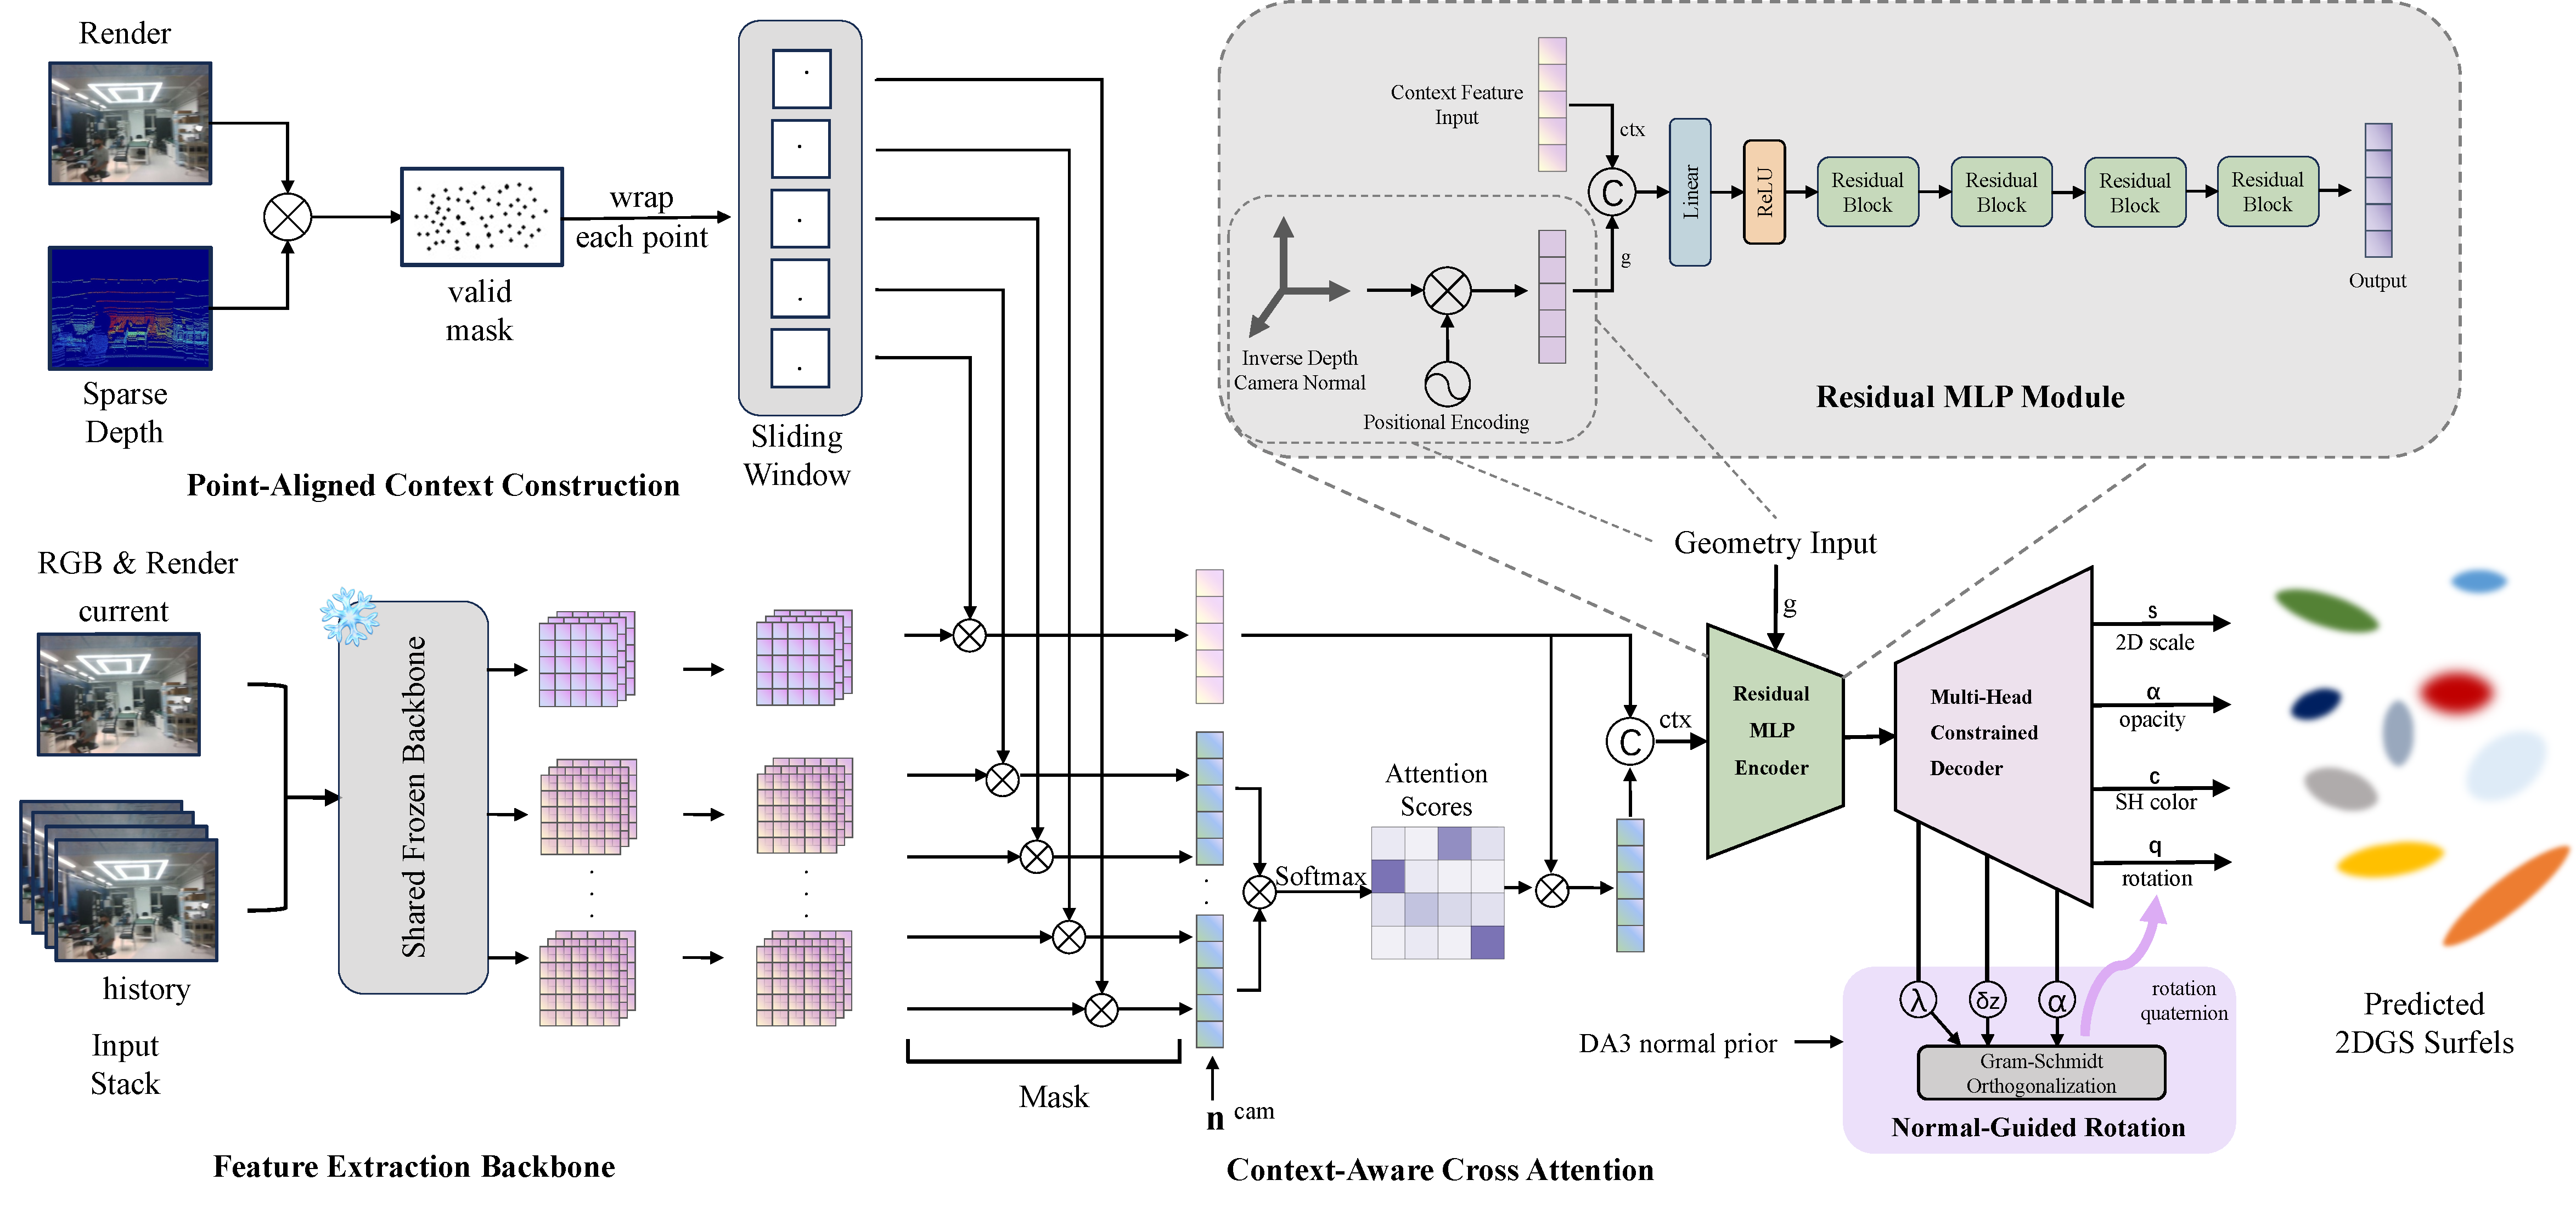
\includegraphics[width=\textwidth,height=0.34\textheight,keepaspectratio]{../../net-pipeline.pdf}
\caption{Architecture of the context-aware feedforward Gaussian regressor. The network first constructs point-aligned context within a sliding window and extracts image-rendering features from the current frame and historical frames using a frozen shared backbone. It then aggregates multiview appearance information with a cross-attention module and combines it with inverse depth, DA3 normals, and positional encoding in a residual MLP encoder. Finally, a multi-head constrained decoder predicts the complete 2DGS surfel attributes $(\mu, s, \alpha, c, q)$, where the normal-guided rotation branch constructs a geometrically consistent orientation through Gram-Schmidt orthogonalization.}
\label{fig:net_pipeline}
\end{figure*}

\subsection{Feedforward Gaussian Regression Network}

This section describes the architecture of the feedforward network in detail. Unlike feedforward Gaussian methods such as MVSplat~\cite{chen2024mvsplat}, which directly recover Gaussian parameters from multiview images, our focus is the setting in which candidate points have already been determined by upstream geometric modules, and the network learns the mapping from point-wise contextual representations and local geometric priors to surfel parameters. For the $N_t$ candidate points selected from the current keyframe, let $\mathbf{ctx}_i$ denote the fused context feature of point $i$ and $\mathbf{g}_i$ its geometric prior vector. The objective of the feedforward network can then be written as

\begin{equation}
f_{\boldsymbol{\theta}} : \{(\mathbf{ctx}_i, \mathbf{g}_i)\}_{i=1}^{N_t}
\mapsto
\{(\mathbf{s}_i, \mathbf{q}_i, \alpha_i, \mathbf{c}_i^{\mathrm{dc}}, \mathbf{c}_i^{\mathrm{rest}})\}_{i=1}^{N_t},
\end{equation}

where the outputs correspond to the surfel's 2D scale, rotation, opacity, and SH color parameters. We now explain how $\mathbf{ctx}_i$ and $\mathbf{g}_i$ are constructed, and how they are encoded and decoded into the final Gaussian attributes.

\methodlead{1) Point-aligned context construction:} The core of input preparation for the feedforward network is point-aligned context construction. Unlike offline pure-vision methods such as pixelSplat~\cite{charatan2024pixelsplat} and MVSplat~\cite{chen2024mvsplat}, which need to infer both geometry and Gaussian attributes from images, our candidate points have already been obtained through LiDAR and depth priors, so the network does not need to implicitly recover position again. The system only needs to explicitly project candidate points into the co-visible window and construct multiview context features at the point level, so that each input vector corresponds one-to-one with a surfel to be inserted.

The feature extraction module follows the backbone design of pixelSplat~\cite{charatan2024pixelsplat}. It projects multiscale ResNet feature layers to a unified dimension through $1 \times 1$ convolutions, upsamples them bilinearly, and sums them to obtain per-pixel feature maps at the same resolution as the input image. To reduce training cost and improve stability, we directly reuse the backbone parameters released by pixelSplat and keep them frozen during training. This shared backbone extracts feature maps from four types of images: the current-frame raw image $I_t \to F_t^{\text{img}}$, the current-frame rendered image $\hat{I}_t \to F_t^{\text{ren}}$ rendered from the current Gaussian map at the current viewpoint, the historical raw images inside the sliding window $\{I_{t-k}\} \to \{F_{t-k}^{\text{img}}\}$, and the historical rendered images $\{\hat{I}_{t-k}\} \to \{F_{t-k}^{\text{ren}}\}$ rendered from the current Gaussian map at historical viewpoints. Introducing rendered images allows the network to perceive the reconstruction status of the current map at that location, and the difference between rendered and raw features implicitly indicates the degree of under-reconstruction in that region.

During current-frame feature sampling, the pixel coordinate $\mathbf{u}_i$ of each candidate point is used to bilinearly sample $F_t^{\text{img}}$ and $F_t^{\text{ren}}$, yielding point-wise features $\mathbf{f}_i^{\text{curr}} \in \mathbb{R}^{D}$ and $\mathbf{f}_i^{\text{ren}} \in \mathbb{R}^{D}$. At the same time, the normalized viewing direction under the current frame is computed as $\mathbf{d}_i^{\text{curr}} = \text{normalize}(R_{\text{cw}} \boldsymbol{\mu}_i + \mathbf{t}_{\text{cw}})$.

During historical-frame projection and feature sampling, for the $W$ historical keyframes inside the co-visible window, the world coordinate of each candidate point is projected frame by frame onto the image plane of each historical frame, visibility is checked (positive depth and inside image bounds), and point-wise historical features $\mathbf{f}_i^{\text{hist}} \in \mathbb{R}^{W \times D}$, historical rendered features $\mathbf{f}_i^{\text{hist\_ren}} \in \mathbb{R}^{W \times D}$, and a visibility mask $\mathbf{m}_i^{\text{hist}} \in \{0,1\}^{W}$ are sampled from $F_{t-k}^{\text{img}}$ and $F_{t-k}^{\text{ren}}$ at the visible pixel locations. We also compute the viewing direction of each frame, expressed in the current-frame coordinate system: $\mathbf{d}_{i,k}^{\text{hist}} = \text{normalize}(R_{\text{cw}}^t (\boldsymbol{\mu}_i - \mathbf{c}_{t-k}))$, where $\mathbf{c}_{t-k}$ is the camera center of the historical frame. This directional encoding is then fed into the attention module together with the historical features.

\methodlead{2) Cross-attention temporal context fusion:} To aggregate the $W$ frames of historical context into a fixed-dimensional temporal context vector, the system uses a single-head cross-attention module. The query vector $\mathbf{q}_i$ is obtained by concatenating the current-frame viewing direction, image feature, and rendered feature followed by a linear projection; the key and value vectors $\mathbf{k}_{i,k}$ and $\mathbf{v}_{i,k}$ are constructed from the corresponding information in each historical frame. The temporal context is computed by masked scaled dot-product attention:

\begin{equation}
\mathbf{ctx}_i^{\text{attn}} = \text{softmax}\!\left(\frac{\mathbf{q}_i \mathbf{K}_i^\top}{\sqrt{d_k}} + \mathbf{M}_i\right) \mathbf{V}_i
\end{equation}

where $d_k = 64$, and $\mathbf{M}_i$ fills the positions of invisible frames with $-\infty$ to fully exclude their contribution. The key idea is that the viewing direction explicitly participates in the projection of queries and keys, so the attention weights can implicitly encode parallax relationships and historical frames close to the current view naturally receive higher weights. Keys and values share the same historical-frame input, so historical information participates in both matching and content aggregation.

\methodlead{3) Geometric input encoding and multi-head prediction decoding:} After obtaining the temporal context, the system concatenates it with the current-frame raw and rendered features to form the context representation of point $i$:
\begin{equation}
\mathbf{ctx}_i = [\mathbf{f}_i^{\text{curr}} \| \mathbf{f}_i^{\text{ren}} \| \mathbf{ctx}_i^{\text{attn}}],
\end{equation}
and concatenates inverse depth, the DA3 camera-space normal, the validity mask, and KNN pixel spacing to form the geometric prior vector
\begin{equation}
\mathbf{g}_i = [\bar{z}_i^{-1} \| \mathbf{n}_i^{\text{cam}} \| m_i \| d_i^{\text{nn}}].
\end{equation}

Before entering the MLP encoder, inverse depth, normals, and pixel spacing are each passed through NeRF-style positional encoding with frequency band counts of 4, 2, and 3, respectively, while the mask $m_i$ remains unchanged. The positional encoding function is $\gamma(v) = [v, \sin(2^0 \pi v), \cos(2^0 \pi v), \ldots, \sin(2^{L-1} \pi v), \cos(2^{L-1} \pi v)]$. The encoded geometric input is
\begin{equation}
\tilde{\mathbf{g}}_i =
[\gamma(\bar{z}_i^{-1}) \| \gamma(\mathbf{n}_i^{\text{cam}}) \| m_i \| \gamma(\log d_i^{\text{nn}})].
\end{equation}

The final network input is
\begin{equation}
\mathbf{x}_i = [\mathbf{ctx}_i \| \tilde{\mathbf{g}}_i].
\end{equation}

The encoder consists of a linear projection from $544 \to 512$ and four pre-activation residual blocks, producing a 512-dimensional feature $\mathbf{h}_i$. On this basis, multiple independent prediction heads regress different attributes in the form $\text{Linear} \to \text{ReLU} \to \text{Linear}$. The outputs of these heads are not used directly as the final Gaussian parameters; instead, they are decoded through geometric constraints, anchoring the network predictions on the upstream geometric priors.

\methodlead{a) Normal-guided rotation construction:} The system does not directly regress quaternions, which are prone to geometric inconsistency in unconstrained space. Instead, it anchors on the camera-space normal $\mathbf{n}_i^{\text{cam}}$ provided by DA3 and predicts correction terms to derive the full rotation through an orthogonalization process.

The network first predicts a normal correction vector $\delta \mathbf{z}_i \in \mathbb{R}^3$, a mixing strength $\lambda_i = \text{softplus}(\cdot) \in \mathbb{R}_{>0}$, and an auxiliary vector $\mathbf{a}_i \in \mathbb{R}^3$, from which the corrected normal direction is obtained:

\begin{equation}
\mathbf{z}_i = \text{normalize}(\mathbf{n}_i^{\text{cam}} + \lambda_i \cdot \delta \mathbf{z}_i)
\end{equation}

The full orthogonal basis is then constructed by Gram-Schmidt orthogonalization using the cross product between the auxiliary vector and the corrected normal:

\begin{equation}
\mathbf{y}_i = \text{normalize}(\mathbf{z}_i \times \mathbf{a}_i), \qquad \mathbf{x}_i = \mathbf{y}_i \times \mathbf{z}_i
\end{equation}

Finally, the camera-space rotation matrix $[\mathbf{x}_i \mid \mathbf{y}_i \mid \mathbf{z}_i]$ is transformed into the world frame by the current-frame pose $R_{\text{wc}}$ and stored as a quaternion. The initialization design ensures that the network starts close to the geometric prior: the bias of the $\lambda$ head is initialized to $-2.0$ (so that $\text{softplus}(-2) \approx 0.13$, making the initial correction magnitude very small), and the bias of the $\mathbf{a}$ head is initialized to $0.1$ (to avoid a degenerate cross product). This guarantees that at the beginning of training, the surfel normal direction is almost entirely determined by the DA3 prior, and the network gradually learns the necessary deviations.

\methodlead{b) Density-adaptive scale prediction:} The network predicts the normalized value of the 2D scale on the pixel plane and adapts it through a local point-density prior:

\begin{equation}
\mathbf{s}_i^{\text{pixel}} = \frac{d_i^{\text{nn}}}{2} \cdot \exp(\text{head}(\mathbf{h}_i)) \in \mathbb{R}^2_{>0}
\end{equation}

where $d_i^{\text{nn}}$ is the KNN pixel spacing of the candidate point. The final world-space scale is obtained via $\mathbf{s}_i^{\text{world}} = \mathbf{s}_i^{\text{pixel}} / (\bar{z}_i^{-1} \cdot f)$. This parameterization allows the network to avoid learning the absolute scale that depends on depth and instead learn only the relative scale associated with local density.

\methodlead{c) Color:} The DC color head outputs a residual $\Delta \mathbf{c}_i^{\text{dc}}$, which is added to the base SH prior converted from the single-frame RGB observation to obtain $\mathbf{c}_i^{\text{dc}} = \text{RGB2SH}(\mathbf{I}_i) + \Delta \mathbf{c}_i^{\text{dc}}$; higher-order SH coefficients are directly predicted by a separate head. This residual design allows the network to start from a reasonable color prior and learn only the correction term.

\methodlead{d) Opacity:} The opacity head outputs the true opacity after sigmoid activation, $\alpha_i = \sigma(\text{head}(\mathbf{h}_i))$, which is then stored in logit space.

\subsection{Self-Distillation Training Loop}

Training of the feedforward network does not depend on an external multiview labeled dataset, but is completed through the following self-distillation pipeline.

\methodlead{1) Online data collection:} The system first runs one complete incremental mapping process on the training scenes in \texttt{naive} mode, which does not use the feedforward network and instead adopts rule-based initialization. During this process, when the accumulated number of optimization steps for newly added Gaussians in a frame reaches the preset threshold, the system snapshots their attributes at that moment as supervision signals; meanwhile, it projects them into the current sliding window and constructs the corresponding context representation $\mathbf{ctx}_i$ and geometric prior vector $\mathbf{g}_i$ as defined above.

Therefore, the collected samples are organized around Gaussians as the core unit, and each training sample can be directly written as the input-output pair $(\mathbf{ctx}_i, \mathbf{g}_i) \mapsto (\mathbf{s}_i, \mathbf{q}_i, \alpha_i, \mathbf{c}_i^{\mathrm{dc}}, \mathbf{c}_i^{\mathrm{rest}})$ defined above.

\methodlead{2) Scale-rotation ambiguity resolution:} 2DGS surfels have an inherent scale-rotation ambiguity: swapping the scales of the two tangent directions and rotating by $90^\circ$ accordingly produces an equivalent representation. If this ambiguity is not resolved, the same geometric shape in the training labels would correspond to two different parameter combinations, causing unstable learning.

This ambiguity is explicitly resolved during data preparation: for each ground-truth Gaussian, we enforce $s_1 \geq s_2$; when a swap is needed, a $90^\circ$ rotation is applied to the quaternion simultaneously: $\mathbf{q}' = \text{normalize}((w-z, x+y, y-x, w+z) / \sqrt{2})$.

\methodlead{3) Training objective:} The network is trained with a multi-task loss covering all predicted attributes, including scale, rotation, color, and opacity. The scale loss is measured by L1 distance in log world-scale space; the rotation loss uses the quaternion cosine distance $\mathcal{L}_{\text{rot}} = 1 - |\langle \mathbf{q}_{\text{pred}}, \mathbf{q}_{\text{gt}} \rangle|$; the color loss supervises the DC and higher-order SH coefficients separately with MSE; and the opacity loss is L1 distance.

\section{Experimental Results}

\subsection{Experimental Setup}
We validate the effectiveness of the proposed method from three aspects. First, we conduct quantitative and qualitative comparisons with MonoGS~\cite{matsuki2024gaussian}, Co-SLAM~\cite{wang2023co}, MM3DGS-SLAM~\cite{sun2024mm3dgs}, and Gaussian-LIC2~\cite{lang2025gaussianlic2} on the public R3LIVE (Avia) dataset~\cite{lin2022r}. Second, we evaluate the generalization capability of the method under a different LiDAR configuration on the MCD (OS1-64) dataset~\cite{nguyen2024mcd}. Third, we further verify the applicability of the method in real new scenes on our self-collected campus dataset. For novel-view rendering quality, we use PSNR, SSIM, and LPIPS as evaluation metrics, where higher is better for PSNR and SSIM, and lower is better for LPIPS. Unless otherwise specified, all methods are evaluated under the same data split, and non-training frames in each sequence are used for sequence-internal novel-view evaluation.

All experiments were carried out in a unified hardware and software environment for system deployment, network training, and new-scene testing. The experimental platform used Ubuntu 20.04 with Python 3.8, implemented in PyTorch 2.0.0 and CUDA 11.8. The hardware configuration consisted of a single RTX 4090D GPU with 24GB memory, an Intel(R) Xeon(R) Platinum 8481C processor with 16 vCPUs, and 80GB of system memory.

The training data for the feedforward regression network came from R3LIVE sequences \texttt{hku\_campus\_seq\_02}, \texttt{hku\_campus\_seq\_03}, \texttt{hkust\_campus\_seq\_02}, and \texttt{hkust\_campus\_seq\_03}, together with our self-collected dataset sequences \texttt{seu\_campus\_seq\_02} and \texttt{seu\_campus\_seq\_03}. Training used the Adam optimizer with batch size 8192 at the point level, together with gradient clipping for stability. The learning rate was fixed to $5\times10^{-4}$, and the total number of epochs was 150. The loss weights were set to $\lambda_{\text{scale}}=1.0$, $\lambda_{\text{rot}}=1.0$, $\lambda_{\text{dc}}=1.0$, $\lambda_{\text{rest}}=0.1$, and $\lambda_{\text{opac}}=1.0$; the camera focal length used in scale recovery was fixed to 431.7103.

It should be emphasized that this set of experiments primarily studies the representation and insertion mechanism of the Gaussian map backend, so the focus is on map rendering quality and the convergence efficiency of newly inserted Gaussians.

\subsection{Comparison with Existing Methods}

Table~\ref{tab:r3live_rendering} reports the quantitative results on the R3LIVE (Avia) dataset~\cite{lin2022r}, the MCD (OS1-64) dataset~\cite{nguyen2024mcd}, and our self-collected campus dataset. For the R3LIVE (Avia) subset, our method achieves the best rendering metrics on all six test sequences. Compared with the closest multisensor baseline Gaussian-LIC2~\cite{lang2025gaussianlic2}, our method improves the average results on these six sequences by \textbf{1.28 dB} PSNR and \textbf{0.041} SSIM, while reducing LPIPS by \textbf{0.030} on average. In the more challenging \texttt{hku\_campus\_01} sequence, the PSNR gain reaches \textbf{2.63 dB}, indicating that the proposed context-aware feedforward insertion strategy can provide more reliable initialization for new Gaussians in difficult viewpoints and degraded regions. For the MCD (OS1-64) subset, the average PSNR and SSIM over the three sequences improve further by approximately \textbf{0.29 dB} and \textbf{0.007}, respectively, compared with Gaussian-LIC2~\cite{lang2025gaussianlic2}, while LPIPS also decreases slightly, showing that the method generalizes stably across different sensor configurations and campus scenes. The same trend is observed on our self-collected campus dataset. On \texttt{seu\_campus\_seq\_00} and \texttt{seu\_campus\_seq\_01}, our method consistently outperforms Gaussian-LIC2, improving PSNR from 23.97 to \textbf{25.55} and from 22.76 to \textbf{24.56}, improving SSIM from 0.769 to \textbf{0.830} and from 0.711 to \textbf{0.797}, and reducing LPIPS from 0.215 to \textbf{0.145} and from 0.195 to \textbf{0.161}. Averaged over the two sequences, this corresponds to a gain of \textbf{1.69 dB} in PSNR, \textbf{0.074} in SSIM, and a reduction of \textbf{0.052} in LPIPS, further supporting the applicability of the proposed feedforward insertion strategy in real campus scenes.

From the perspective of individual methods, the purely visual MonoGS~\cite{matsuki2024gaussian} suffers from obvious blur, floating artifacts, and structural collapse in large-scale outdoor and degraded scenes, which shows that it is very difficult to correct inaccurate initialization only through subsequent optimization. After adding LiDAR geometric priors, Gaussian-LIC2~\cite{lang2025gaussianlic2} already achieves a significant improvement overall, but its new Gaussian attributes still mainly depend on rule-based design, so drag, excessive smoothing, and local distortion remain in bright regions, boundary regions, and poorly observed regions. In contrast, our method uses image-rendering context from the current and historical frames to provide surfels with attributes that are closer to the converged state at insertion time, so that subsequent limited optimization can produce more stable appearance and clearer structure.

\begin{table*}[!t]
\centering
\caption{Comparison of sequence-wise novel-view RGB rendering results on the public R3LIVE (Avia), MCD (OS1-64), and our self-collected campus dataset. The evaluation format is PSNR$\uparrow$ SSIM$\uparrow$ LPIPS$\downarrow$.}
\label{tab:r3live_rendering}
\renewcommand{\arraystretch}{1.15}
\setlength{\tabcolsep}{8pt}
\resizebox{\textwidth}{!}{%
\begin{tabular}{lcccc}
\toprule
\textbf{Sequence} & \multicolumn{4}{c}{\textbf{Rendering Performance (PSNR$\uparrow$ SSIM$\uparrow$ LPIPS$\downarrow$)}} \\
\cmidrule(lr){2-5}
& \textbf{MonoGS} & \textbf{MM3DGS-SLAM} & \textbf{Gaussian-LIC2} & \textbf{Ours} \\
\midrule
\rowcolor{black!8}
\multicolumn{5}{l}{\textbf{R3LIVE (Avia)}} \\
degenerate\_seq\_00 & 14.59 \textbar{} 0.460 \textbar{} 0.624 & 19.35 \textbar{} 0.698 \textbar{} 0.212 & 21.99 \textbar{} 0.782 \textbar{} 0.162 & \textbf{23.41} \textbar{} \textbf{0.821} \textbar{} \textbf{0.137} \\
degenerate\_seq\_01 & 14.66 \textbar{} 0.438 \textbar{} 0.692 & 18.57 \textbar{} 0.621 \textbar{} 0.277 & 22.94 \textbar{} 0.790 \textbar{} 0.159 & \textbf{23.54} \textbar{} \textbf{0.810} \textbar{} \textbf{0.157} \\
hku\_campus\_00 & 15.41 \textbar{} 0.464 \textbar{} 0.675 & 18.70 \textbar{} 0.621 \textbar{} 0.319 & 24.34 \textbar{} 0.787 \textbar{} 0.156 & \textbf{25.52} \textbar{} \textbf{0.820} \textbar{} \textbf{0.152} \\
hku\_campus\_01 & 8.39 \textbar{} 0.065 \textbar{} 0.873 & 16.97 \textbar{} 0.593 \textbar{} 0.271 & 20.52 \textbar{} 0.674 \textbar{} 0.236 & \textbf{23.15} \textbar{} \textbf{0.754} \textbar{} \textbf{0.174} \\
hku\_park\_00 & 13.24 \textbar{} 0.319 \textbar{} 0.733 & 14.98 \textbar{} 0.363 \textbar{} 0.396 & 17.17 \textbar{} 0.469 \textbar{} 0.340 & \textbf{17.80} \textbar{} \textbf{0.491} \textbar{} \textbf{0.331} \\
hku\_park\_01 & 12.22 \textbar{} 0.289 \textbar{} 0.790 & 15.79 \textbar{} 0.392 \textbar{} 0.409 & 19.46 \textbar{} 0.529 \textbar{} 0.325 & \textbf{20.65} \textbar{} \textbf{0.580} \textbar{} \textbf{0.248} \\
\rowcolor{black!8}
\multicolumn{5}{l}{\textbf{MCD (OS1-64)}} \\
tuhh\_day\_02 & 8.72 \textbar{} 0.158 \textbar{} 0.893 & 11.15 \textbar{} 0.478 \textbar{} 0.350 & 20.35 \textbar{} 0.626 \textbar{} 0.262 & \textbf{20.99} \textbar{} \textbf{0.652} \textbar{} \textbf{0.249} \\
tuhh\_day\_03 & 8.09 \textbar{} 0.136 \textbar{} 0.896 & 11.36 \textbar{} 0.542 \textbar{} 0.301 & 21.38 \textbar{} 0.672 \textbar{} \textbf{0.229} & \textbf{21.82} \textbar{} \textbf{0.688} \textbar{} 0.238 \\
tuhh\_day\_04 & 11.73 \textbar{} 0.250 \textbar{} 0.805 & 13.86 \textbar{} 0.384 \textbar{} 0.398 & \textbf{19.27} \textbar{} \textbf{0.528} \textbar{} 0.310 & 19.07 \textbar{} 0.506 \textbar{} \textbf{0.309} \\
\rowcolor{black!8}
\multicolumn{5}{l}{\textbf{Self-Collected Campus Dataset}} \\
seu\_campus\_seq\_00 & 14.56 \textbar{} 0.411 \textbar{} 0.732 & 18.54 \textbar{} 0.563 \textbar{} 0.366 & 23.97 \textbar{} 0.769 \textbar{} 0.215 & \textbf{25.55} \textbar{} \textbf{0.830} \textbar{} \textbf{0.145} \\
seu\_campus\_seq\_01 & 13.21 \textbar{} 0.392 \textbar{} 0.796 & 17.14 \textbar{} 0.528 \textbar{} 0.421 & 22.76 \textbar{} 0.711 \textbar{} 0.195 & \textbf{24.56} \textbar{} \textbf{0.797} \textbar{} \textbf{0.161} \\
\bottomrule
\end{tabular}%
}
\end{table*}

\begin{figure*}[t]
\centering
\setlength{\tabcolsep}{2pt}
\begin{tabular}{ccccc}
\small GT & \small MonoGS & \small MM3DGS-SLAM & \small Gaussian-LIC2 & \small Ours \\
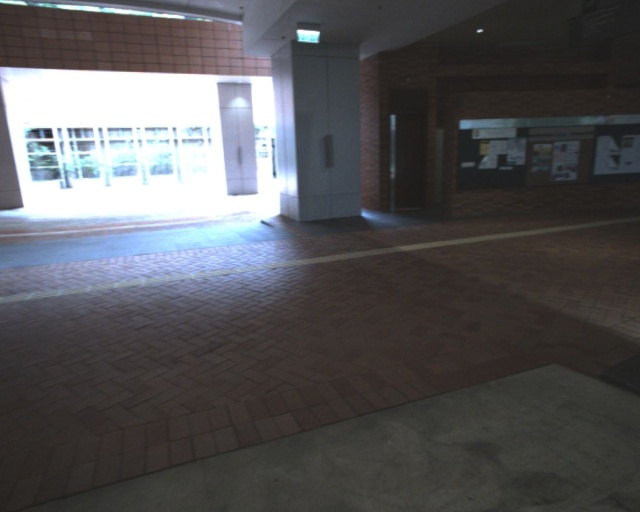
\includegraphics[width=0.188\textwidth]{../../../images/compare-hku_campus_00/gt/test_0690.jpg} &
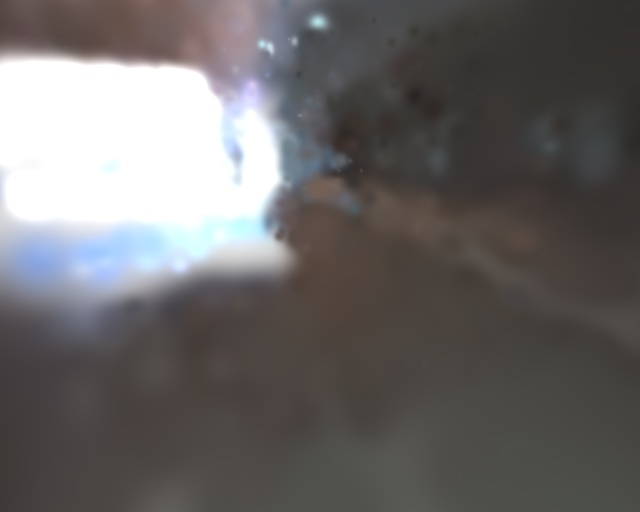
\includegraphics[width=0.188\textwidth]{../../../images/compare-hku_campus_00/monogs/0690-test.jpg} &
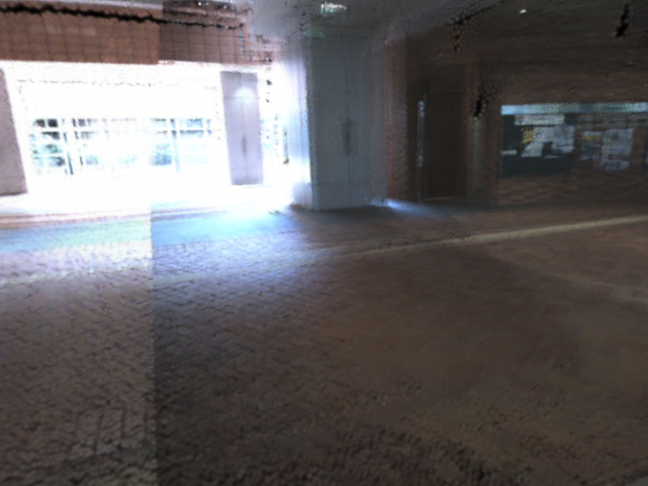
\includegraphics[width=0.188\textwidth]{../../../images/compare-hku_campus_00/mm3dgs/test_0690.png} &
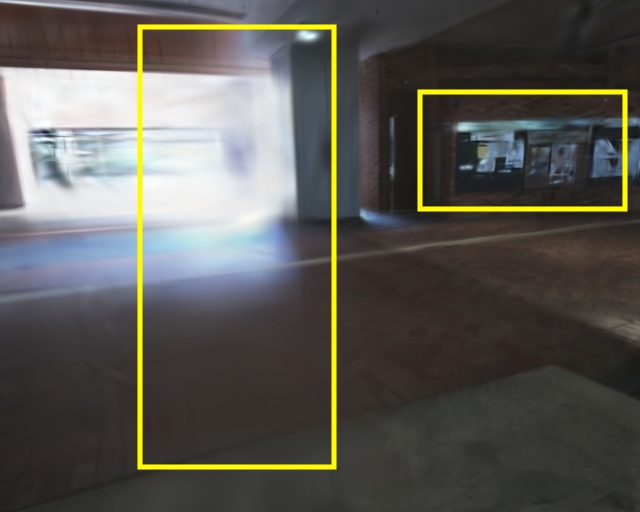
\includegraphics[width=0.188\textwidth]{../../../images/compare-hku_campus_00/gslic2/test_0690.jpg} &
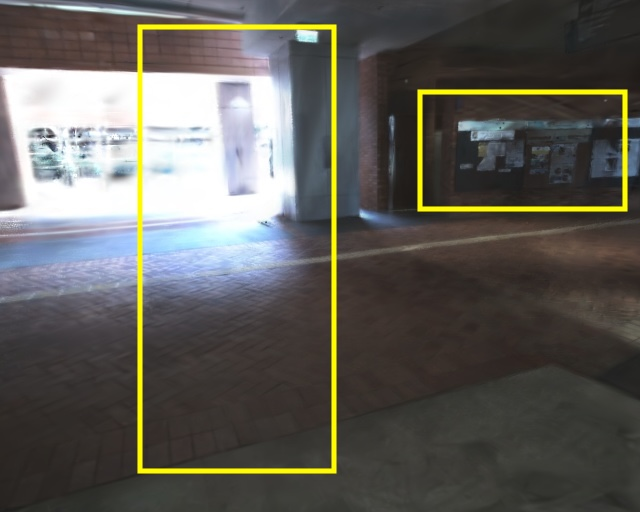
\includegraphics[width=0.188\textwidth]{../../../images/compare-hku_campus_00/ours/test_0690.jpg} \\
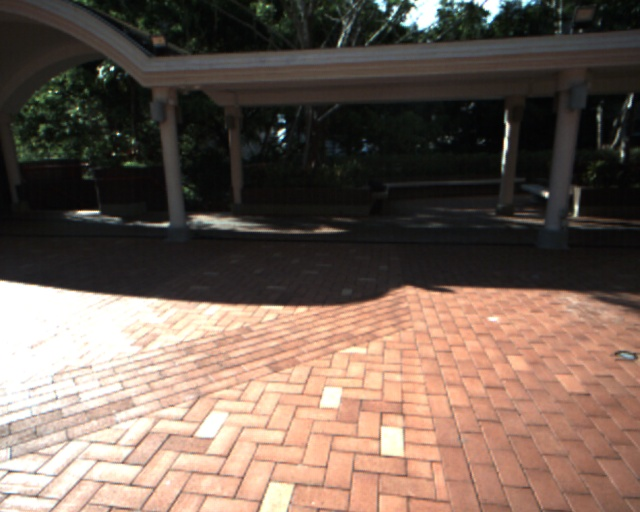
\includegraphics[width=0.188\textwidth]{../../../images/compare-degenerate_00/gt/test_0516.jpg} &
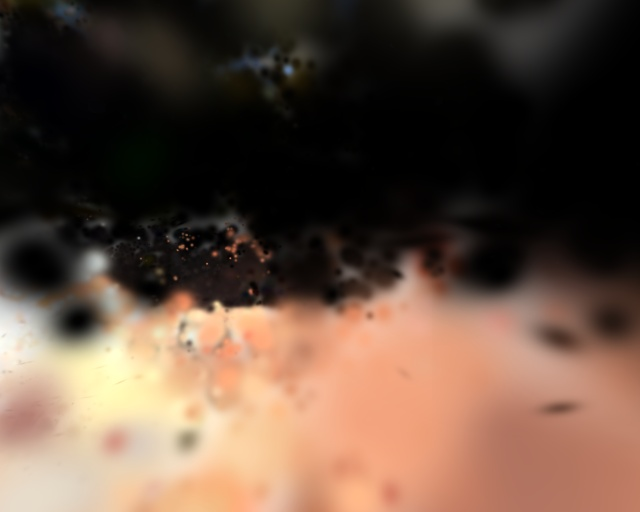
\includegraphics[width=0.188\textwidth]{../../../images/compare-degenerate_00/monogs/0516-test.jpg} &
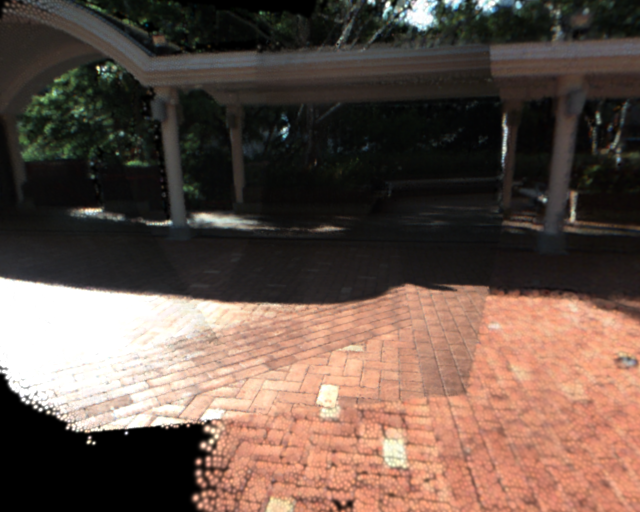
\includegraphics[width=0.188\textwidth]{../../../images/compare-degenerate_00/mm3dgs/test_0516.png} &
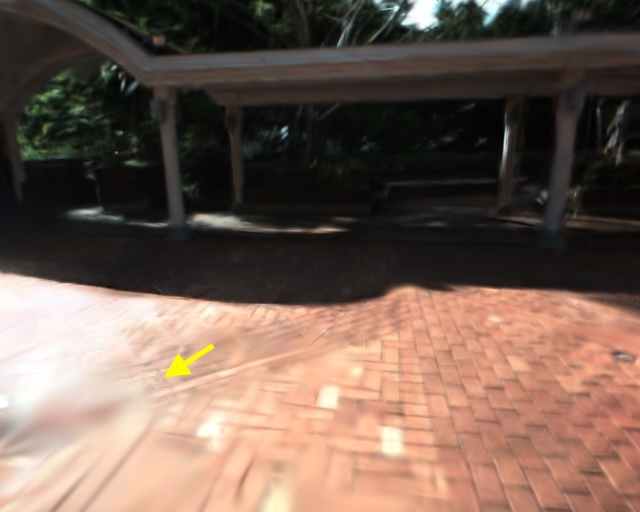
\includegraphics[width=0.188\textwidth]{../../../images/compare-degenerate_00/gslic2/test_0516.jpg} &
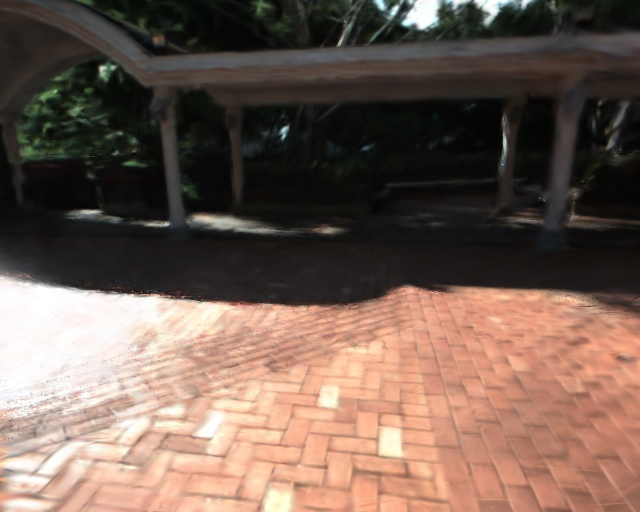
\includegraphics[width=0.188\textwidth]{../../../images/compare-degenerate_00/ours/test_0516.jpg} \\
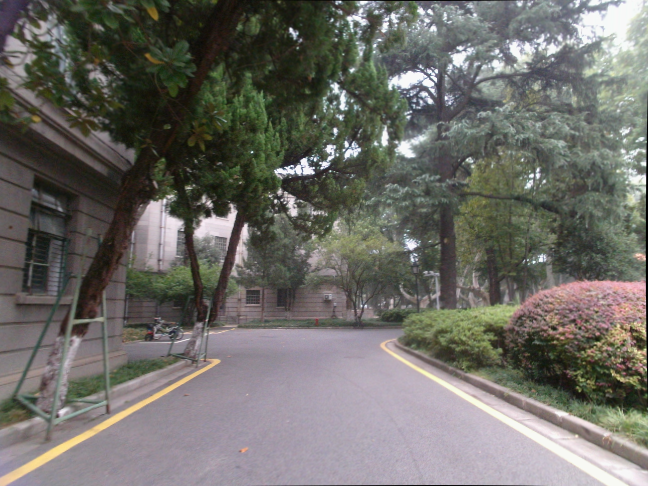
\includegraphics[width=0.188\textwidth]{../../../images/compare-custom-2/gt/test_1080.png} &
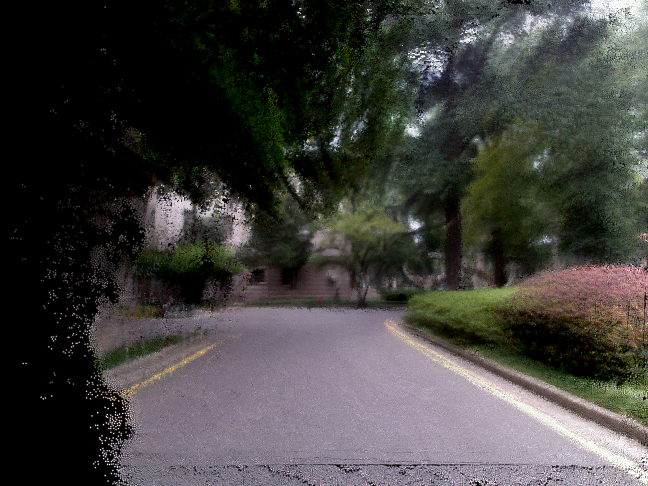
\includegraphics[width=0.188\textwidth]{../../../images/compare-custom-2/monogs/test_1080.jpg} &
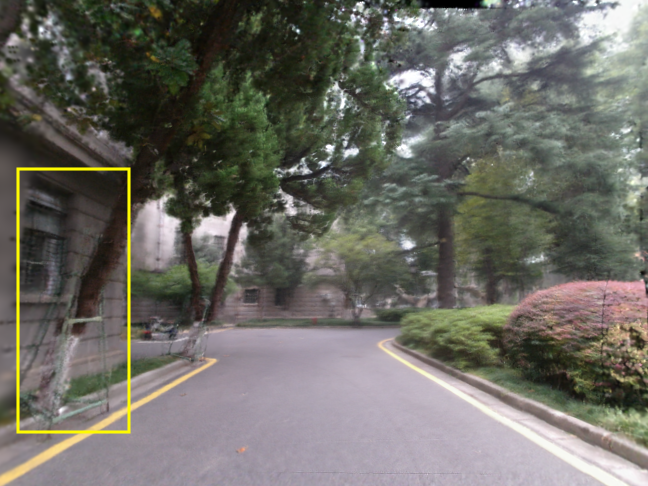
\includegraphics[width=0.188\textwidth]{../../../images/compare-custom-2/mm3dgs/test_1080.png} &
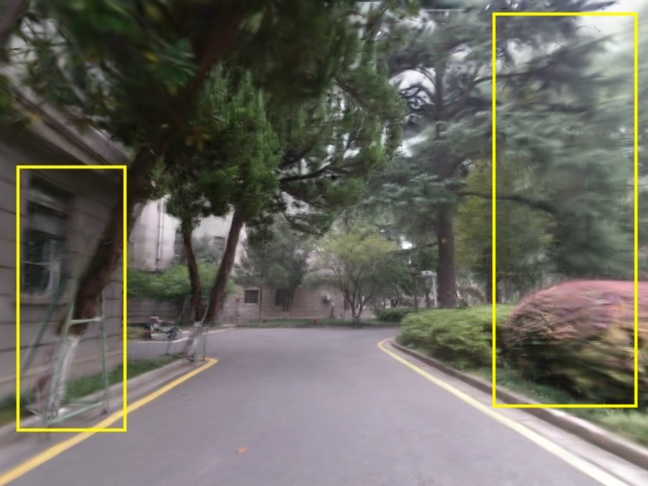
\includegraphics[width=0.188\textwidth]{../../../images/compare-custom-2/gslic2/test_1080.jpg} &
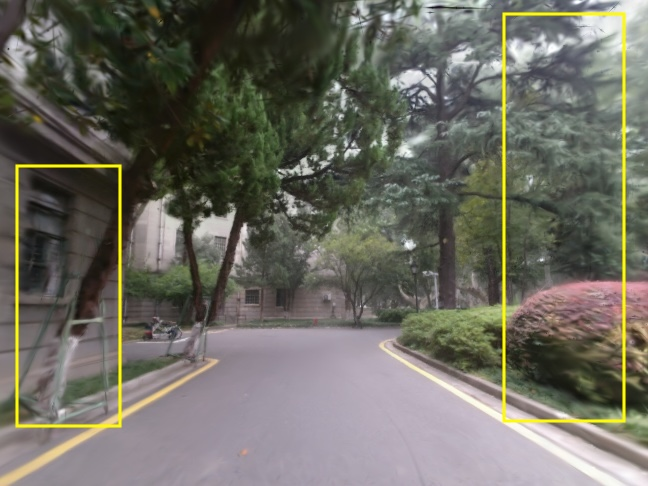
\includegraphics[width=0.188\textwidth]{../../../images/compare-custom-2/ours/test_1080.jpg} \\
\end{tabular}
\caption{Qualitative comparison results on both public and self-collected datasets. The first row shows frame 690 of \texttt{hku\_campus\_00}, the second row shows frame 516 of \texttt{degenerate\_seq\_00}, and the third row shows frame 1080 of \texttt{seu\_campus\_seq\_01}. Compared with MonoGS, MM3DGS-SLAM, and Gaussian-LIC2, our method preserves clearer structures and textures while significantly reducing blur, drag, and local distortion.}
\label{fig:qualitative_compare}
\end{figure*}

Figure~\ref{fig:qualitative_compare} presents three representative qualitative results. For the indoor-outdoor transition scene in \texttt{hku\_campus\_00}, MonoGS fails to recover a stable structure almost entirely, and MM3DGS-SLAM still exhibits noticeably over-smoothed structures and weakened boundary sharpness. Gaussian-LIC2 reconstructs the main geometric outline but still shows obvious blur and edge softness near the strongly exposed exit and the right-side pillar region. In contrast, our method better preserves the floor-tile texture and pillar contour. In the \texttt{degenerate\_seq\_00} scene, MonoGS exhibits large-scale collapse and incorrect color accumulation, MM3DGS-SLAM recovers more structure but still suffers from noticeable distortion in difficult regions, and Gaussian-LIC2 still shows strong drag in the bright region at the lower left. In the self-collected \texttt{seu\_campus\_seq\_01} scene, MonoGS produces obvious blur and structural degradation, MM3DGS-SLAM recovers a more complete layout but still loses fine details around distant building edges, and Gaussian-LIC2 still shows smoothing and local distortion on facade boundaries and textured ground areas. Our method remains superior in overall clarity, structural sharpness, and local consistency across all three scenes.

\subsection{Ablation Study: The Role of the Feedforward Regressor}

To verify the contribution of the feedforward regressor to incremental 2DGS mapping, we conducted ablation experiments on the \texttt{hku\_campus\_00} sequence. Here, the system without the regressor and using rule-based initialization is denoted as \textbf{Baseline}, and the system with the context-aware feedforward regressor is denoted as \textbf{Ours}. Unlike a comparison on only a few representative frames, we statistically analyze all optimization trajectories of the training frames and use the number of local optimization steps after Gaussian insertion (\texttt{train\_times}) as the horizontal axis, evaluating the regressor from three perspectives: 1) early quality under a fixed optimization budget; 2) overall convergence gain within the first 16 rounds; and 3) the number of optimization rounds required to reach a given quality threshold.

\begin{table}[!t]
\centering
\caption{Feedforward regressor ablation on \texttt{hku\_campus\_00}.}
\label{tab:ablation_regressor}
\renewcommand{\arraystretch}{1.18}
\resizebox{\columnwidth}{!}{%
\begin{tabular}{lccc}
\toprule
\textbf{Setting} & \textbf{PSNR$\uparrow$} & \textbf{SSIM$\uparrow$} & \textbf{LPIPS$\downarrow$} \\
\midrule
Baseline (16 rounds) & 23.97 $\pm$ 2.91 & 0.800 $\pm$ 0.071 & 0.213 $\pm$ 0.055 \\
Ours (16 rounds) & \textbf{24.34 $\pm$ 2.74} & \textbf{0.813 $\pm$ 0.063} & \textbf{0.195 $\pm$ 0.048} \\
\midrule
Baseline (AUC@16) & 362.96 $\pm$ 44.54 & 12.251 $\pm$ 1.302 & 4.266 $\pm$ 0.978 \\
Ours (AUC@16) & \textbf{370.57 $\pm$ 40.43} & \textbf{12.475 $\pm$ 1.149} & \textbf{4.033 $\pm$ 0.866} \\
\midrule
Baseline (time-to-quality) & 20.4 $\pm$ 28.1 (255/391) & 3.2 $\pm$ 6.2 (373/391) & 27.0 $\pm$ 24.5 (257/391) \\
Ours (time-to-quality) & \textbf{17.7 $\pm$ 26.0 (281/391)} & \textbf{3.1 $\pm$ 10.2 (382/391)} & \textbf{19.6 $\pm$ 15.6 (323/391)} \\
\bottomrule
\end{tabular}%
}
\end{table}

Table~\ref{tab:ablation_regressor} shows that introducing the feedforward regressor stably improves the overall early convergence behavior on the training frames. First, under the fixed budget of 16 rounds of local optimization, Ours outperforms Baseline on all three metrics: PSNR increases from 23.97 $\pm$ 2.91 to 24.34 $\pm$ 2.74, SSIM increases from 0.800 $\pm$ 0.071 to 0.813 $\pm$ 0.063, and LPIPS decreases from 0.213 $\pm$ 0.055 to 0.195 $\pm$ 0.048. Since this statistic only includes training frames that completed at least 16 rounds of local optimization, it more directly reflects the average quality of newly inserted Gaussians under a fixed early budget.

Second, from the AUC statistics over the first 16 rounds, Ours is better on all three metrics: PSNR AUC increases from 362.96 $\pm$ 44.54 to 370.57 $\pm$ 40.43, SSIM AUC increases from 12.251 $\pm$ 1.302 to 12.475 $\pm$ 1.149, and LPIPS AUC decreases from 4.266 $\pm$ 0.978 to 4.033 $\pm$ 0.866. Since AUC measures the accumulated rendering quality over the entire early optimization stage, this means the advantage of our method is not limited to a single sampling round but appears as a more stable overall convergence gain.

Furthermore, we use fixed quality thresholds to evaluate how many local optimization rounds are needed for the two methods to reach "usable quality", where the thresholds for PSNR, SSIM, and LPIPS are set to 25.0, 0.70, and 0.18, respectively. The results show that Ours reaches the target quality with fewer average optimization rounds on all three metrics: the corresponding numbers decrease from 20.4 $\pm$ 28.1, 3.2 $\pm$ 6.2, and 27.0 $\pm$ 24.5 to 17.7 $\pm$ 26.0, 3.1 $\pm$ 10.2, and 19.6 $\pm$ 15.6. At the same time, Ours also achieves higher coverage counts under the three thresholds, reaching 281/391, 382/391, and 323/391, whereas Baseline reaches 255/391, 373/391, and 257/391. This indicates that the feedforward regressor not only improves average early quality, but also increases the probability that more training frames reach the target quality within a limited local optimization budget. To visualize this stable advantage in the early stage more directly, Fig.~\ref{fig:ablation_curves} further summarizes the mean convergence trends of the three metrics over the first 16 local optimization steps after insertion.

\begin{figure}[!t]
\centering
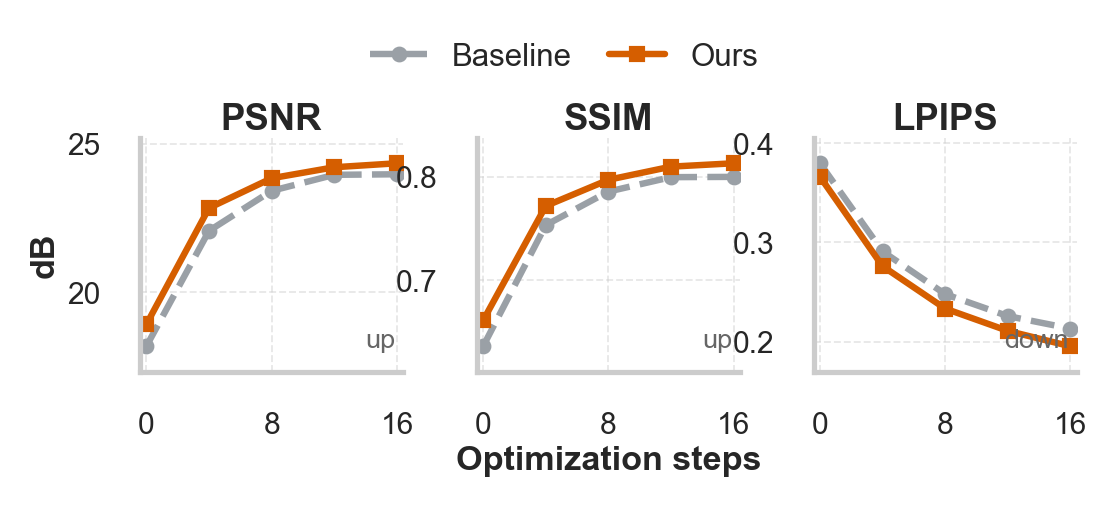
\includegraphics[width=\columnwidth]{../../../analysis_outputs/self_compare-3/figs/ablation_curves_paper_compact_demo.png}% compact version: ablation_curves_paper_compact_demo.png
\caption{Early convergence comparison of the feedforward regressor ablation. From left to right, the plots show the mean PSNR, SSIM, and LPIPS curves over the first 16 local optimization steps after insertion, highlighting the early-stage difference between Baseline and Ours.}
\label{fig:ablation_curves}
\end{figure}

Figure~\ref{fig:ablation_curves} further shows that Ours typically achieves higher PSNR and SSIM and lower LPIPS in the first few local optimization rounds, with smaller overall fluctuations. This is consistent with the quantitative results in Table~\ref{tab:ablation_regressor}, indicating that the benefits brought by the feedforward regressor can be stably observed throughout the early optimization process of the training frames.

The complete visual results in Fig.~\ref{fig:ablation_visual_1} and Fig.~\ref{fig:ablation_visual_2} are moved to the appendix so that the main text can focus on quantitative analysis and early convergence curves. The corresponding figures still retain the initialization differences and local optimization process of representative frames, making it easier to further inspect the effect of the feedforward regressor on the initial state of new Gaussians.

\subsection{Discussion}

Two conclusions can be drawn from the above experiments. First, in the full novel-view rendering evaluation, our method outperforms the existing baselines on all test sequences, showing that the combination of 2DGS representation and context-aware feedforward insertion can stably improve the rendering quality of incremental Gaussian maps. Second, the core value of the feedforward regressor is not merely a slightly higher final score; more importantly, it significantly improves the initial quality and early convergence speed of newly inserted Gaussians. This is particularly important for online systems, because better initial Gaussians not only reduce local artifacts but also provide more reliable rendering supervision for subsequent frames, forming a positive loop that continuously improves the mapping quality of the entire scene.

\section{Conclusion}

For the problem that the initial quality of newly inserted Gaussians determines the accumulated quality of the map in incremental scene reconstruction, this paper proposes a context-aware feedforward Gaussian regression system based on 2DGS surfels. The method combines geometric priors with multiview image-rendering context and directly predicts the complete attributes of new surfels at insertion time, replacing conventional rule-based initialization. At the same time, the network can be trained through a self-distillation loop without additional labeled data.

Experiments on the R3LIVE, MCD, and self-collected campus datasets show that the proposed method can stably improve the novel-view rendering quality of incremental Gaussian maps, and achieves an average gain of 1.28\,dB PSNR on R3LIVE compared with the closest multisensor baseline. Ablation experiments further show that the main benefit of the method comes from improving the initial state and early convergence quality of new surfels, which is especially important for online mapping under a limited optimization budget. The current method still relies on an external stable front end, and future work will further explore incremental Gaussian mapping under weaker prior conditions.

% \clearpage
\bibliographystyle{IEEEtran}
\bibliography{references}
% \clearpage
% \appendix[Visualizations of Feedforward Regressor Ablation]
% \clearpage

\begin{figure*}[!b]
\centering
\setlength{\tabcolsep}{2pt}
\begin{tabular}{cccc}
& \small 0 Optimization Steps & \small 4 Optimization Steps & \small 8 Optimization Steps \\
\rotatebox{90}{Baseline} &
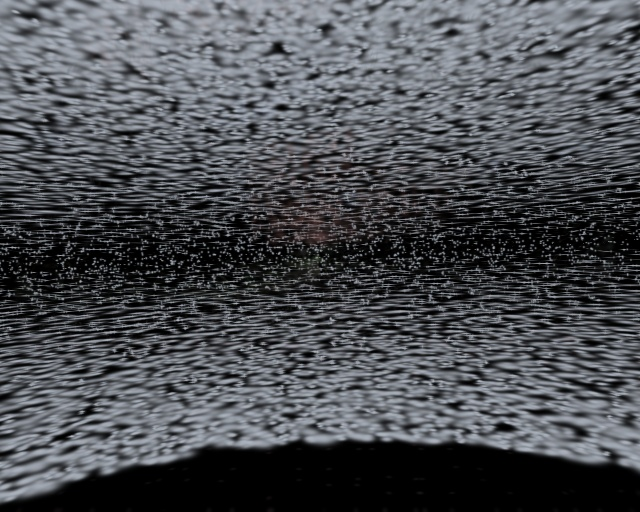
\includegraphics[width=0.30\textwidth]{../../../images/self_compare/baseline/train_0004/times_0000.jpg} &
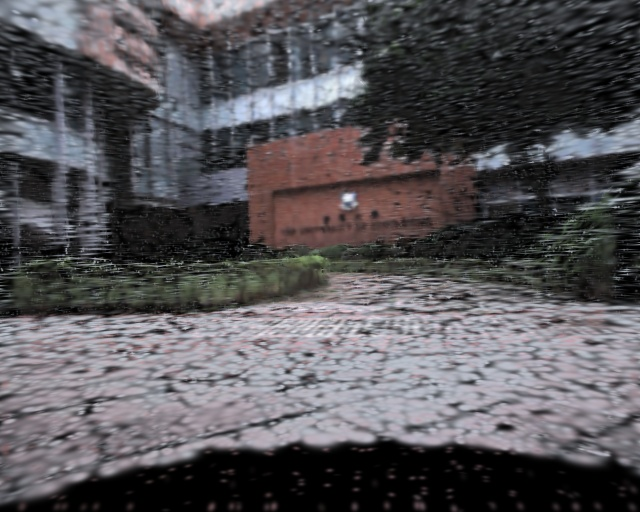
\includegraphics[width=0.30\textwidth]{../../../images/self_compare/baseline/train_0004/times_0004.jpg} &
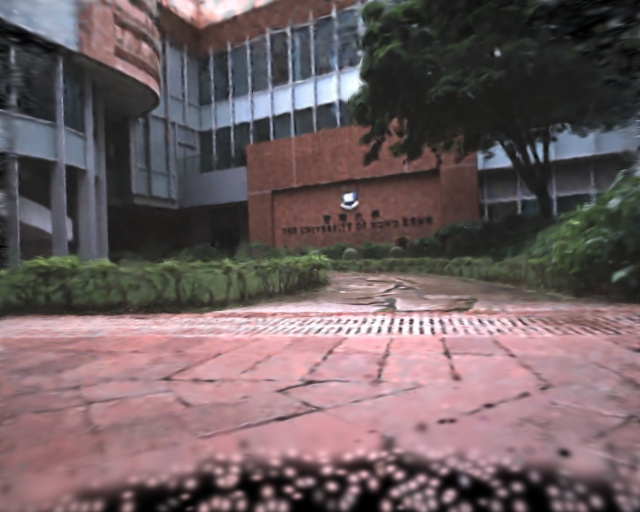
\includegraphics[width=0.30\textwidth]{../../../images/self_compare/baseline/train_0004/times_0008.jpg} \\
\rotatebox{90}{Ours} &
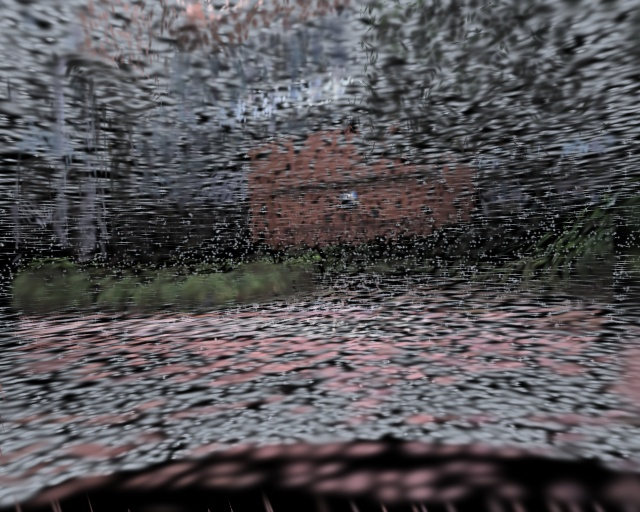
\includegraphics[width=0.30\textwidth]{../../../images/self_compare/ours/train_0004/times_0000.jpg} &
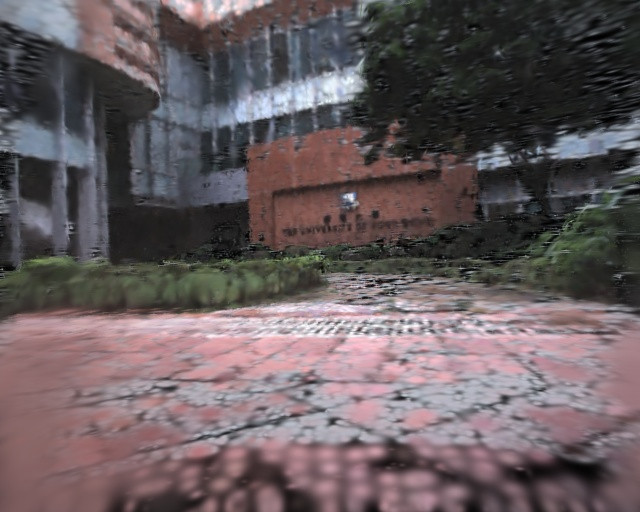
\includegraphics[width=0.30\textwidth]{../../../images/self_compare/ours/train_0004/times_0004.jpg} &
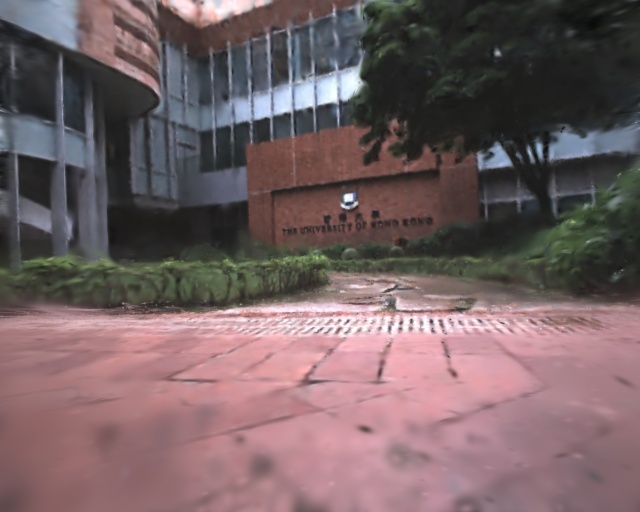
\includegraphics[width=0.30\textwidth]{../../../images/self_compare/ours/train_0004/times_0008.jpg} \\
\rotatebox{90}{Baseline} &
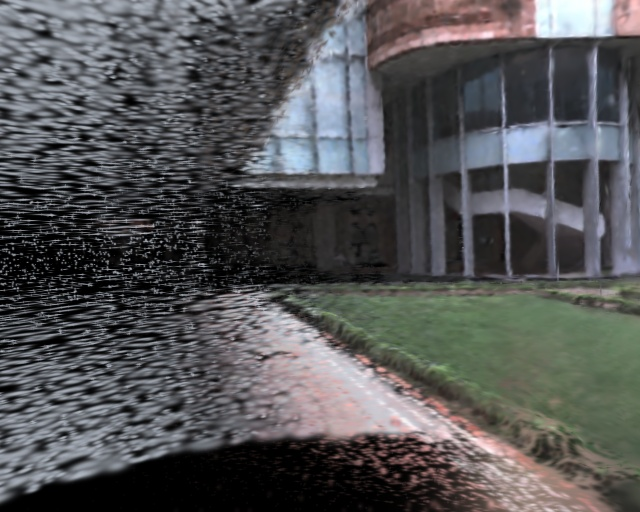
\includegraphics[width=0.30\textwidth]{../../../images/self_compare/baseline/train_0084/times_0000.jpg} &
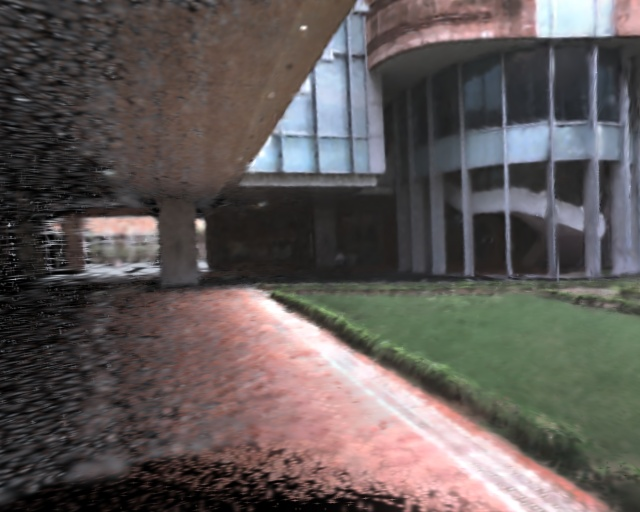
\includegraphics[width=0.30\textwidth]{../../../images/self_compare/baseline/train_0084/times_0004.jpg} &
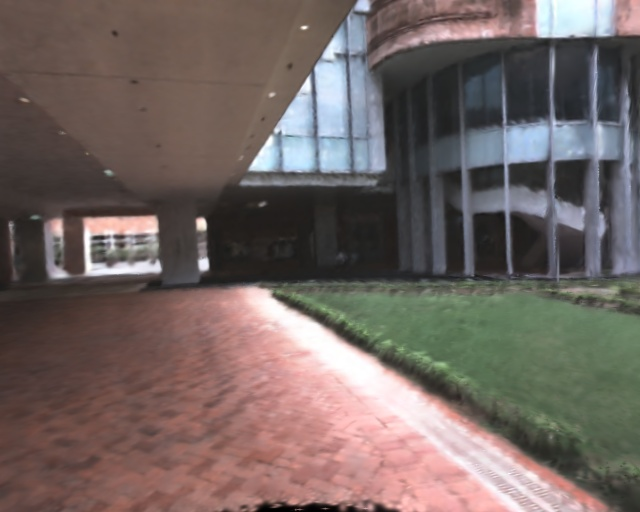
\includegraphics[width=0.30\textwidth]{../../../images/self_compare/baseline/train_0084/times_0008.jpg} \\
\rotatebox{90}{Ours} &
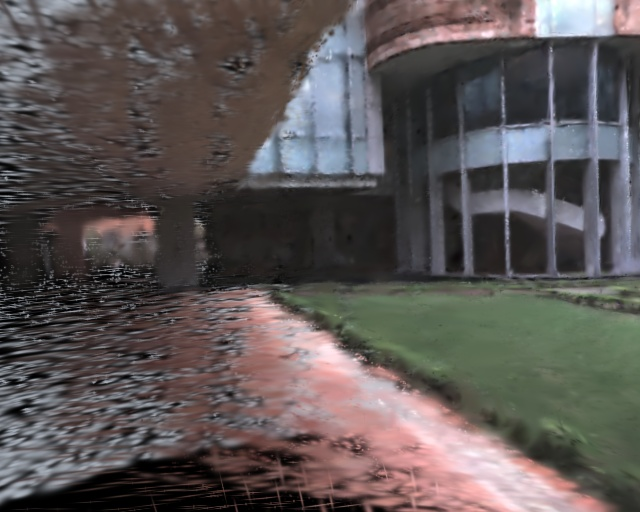
\includegraphics[width=0.30\textwidth]{../../../images/self_compare/ours/train_0084/times_0000.jpg} &
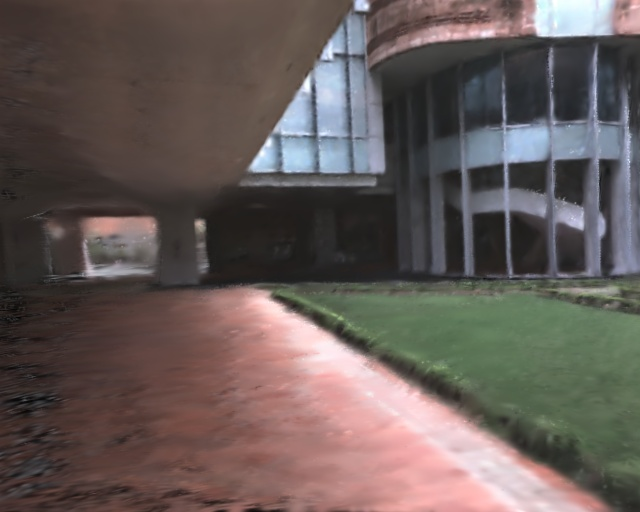
\includegraphics[width=0.30\textwidth]{../../../images/self_compare/ours/train_0084/times_0004.jpg} &
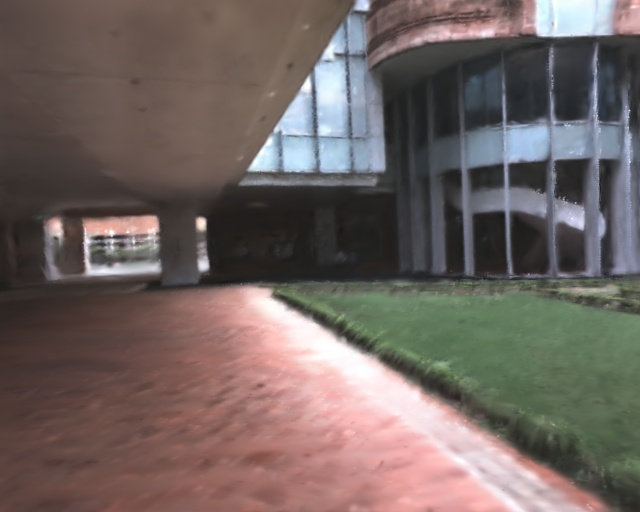
\includegraphics[width=0.30\textwidth]{../../../images/self_compare/ours/train_0084/times_0008.jpg} \\
\end{tabular}
\caption{Visualization results of the feedforward regressor ablation (I). The figure shows the rendered results of representative frames \texttt{train\_0004} and \texttt{train\_0084} in \texttt{hku\_campus\_00} after 0, 4, and 8 local optimization steps. For each representative frame, the first two rows are Baseline and the last two rows are Ours.}
\label{fig:ablation_visual_1}
\end{figure*}

\begin{figure*}[t]
\centering
\setlength{\tabcolsep}{2pt}
\begin{tabular}{cccc}
& \small 0 Optimization Steps & \small 4 Optimization Steps & \small 8 Optimization Steps \\
\rotatebox{90}{Baseline} &
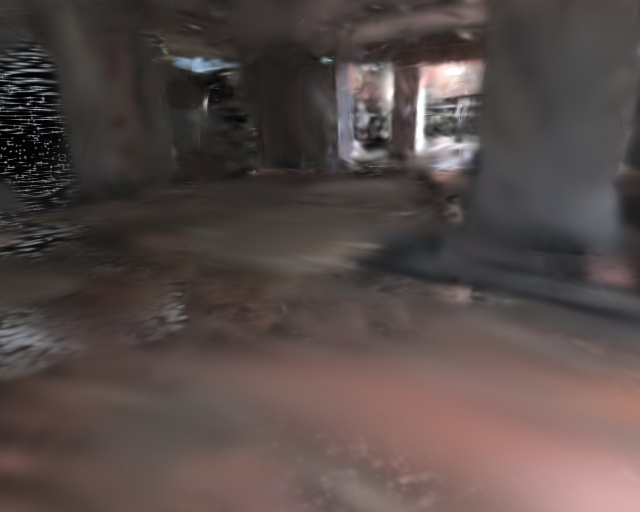
\includegraphics[width=0.30\textwidth]{../../../images/self_compare/baseline/train_0609/times_0000.jpg} &
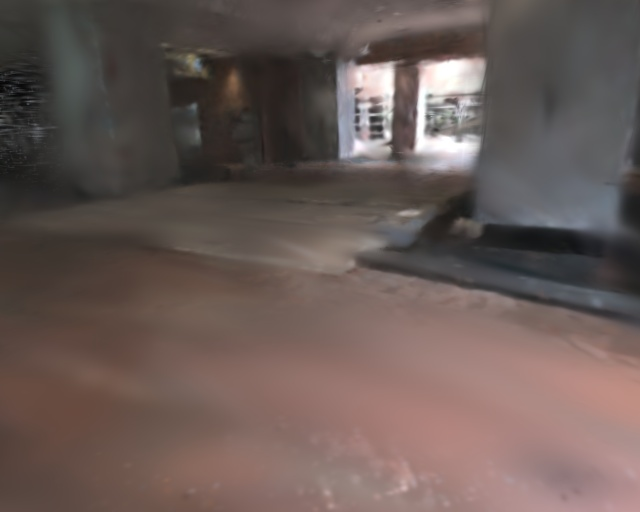
\includegraphics[width=0.30\textwidth]{../../../images/self_compare/baseline/train_0609/times_0004.jpg} &
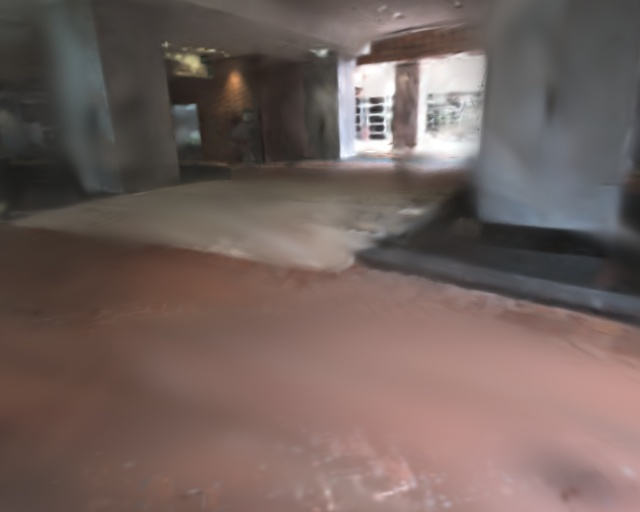
\includegraphics[width=0.30\textwidth]{../../../images/self_compare/baseline/train_0609/times_0008.jpg} \\
\rotatebox{90}{Ours} &
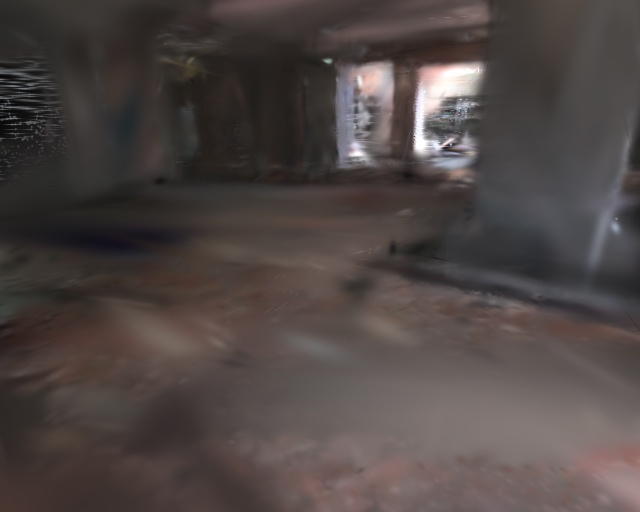
\includegraphics[width=0.30\textwidth]{../../../images/self_compare/ours/train_0609/times_0000.jpg} &
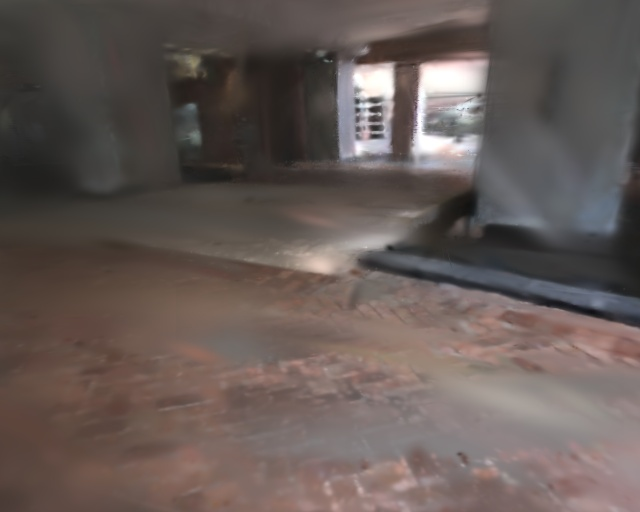
\includegraphics[width=0.30\textwidth]{../../../images/self_compare/ours/train_0609/times_0004.jpg} &
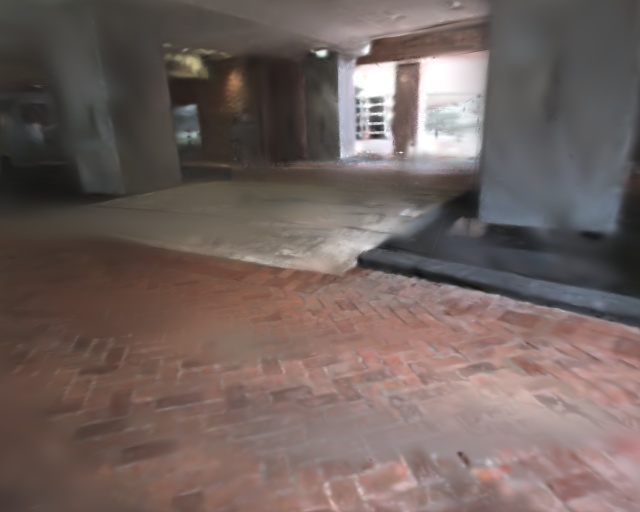
\includegraphics[width=0.30\textwidth]{../../../images/self_compare/ours/train_0609/times_0008.jpg} \\
\rotatebox{90}{Baseline} &
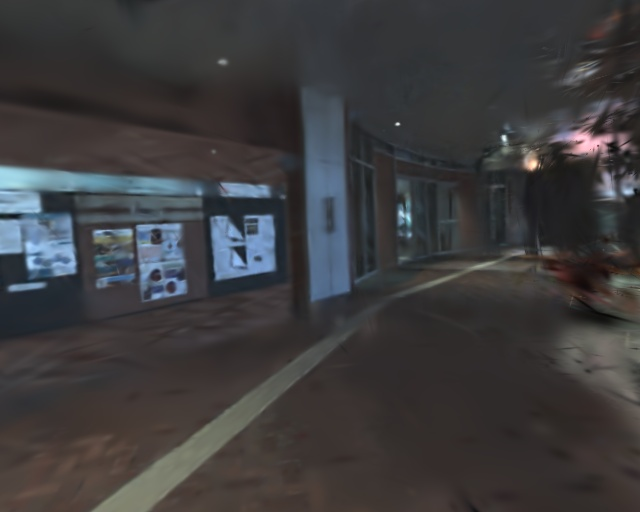
\includegraphics[width=0.30\textwidth]{../../../images/self_compare/baseline/train_0784/times_0000.jpg} &
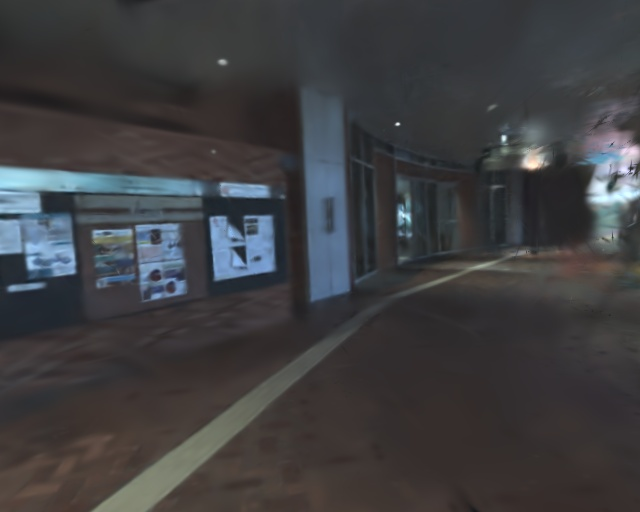
\includegraphics[width=0.30\textwidth]{../../../images/self_compare/baseline/train_0784/times_0004.jpg} &
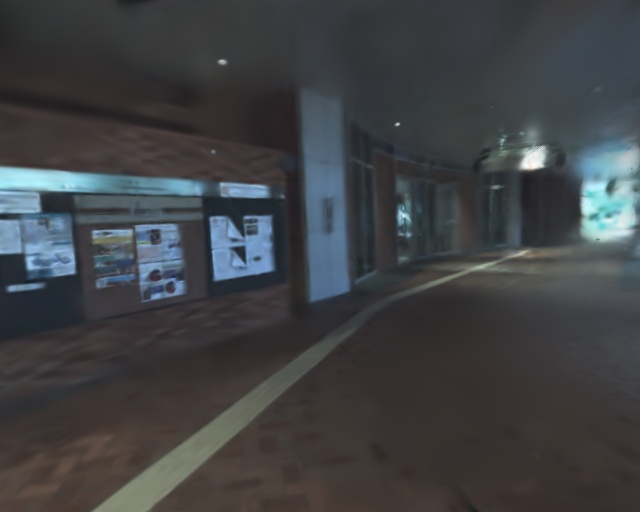
\includegraphics[width=0.30\textwidth]{../../../images/self_compare/baseline/train_0784/times_0008.jpg} \\
\rotatebox{90}{Ours} &
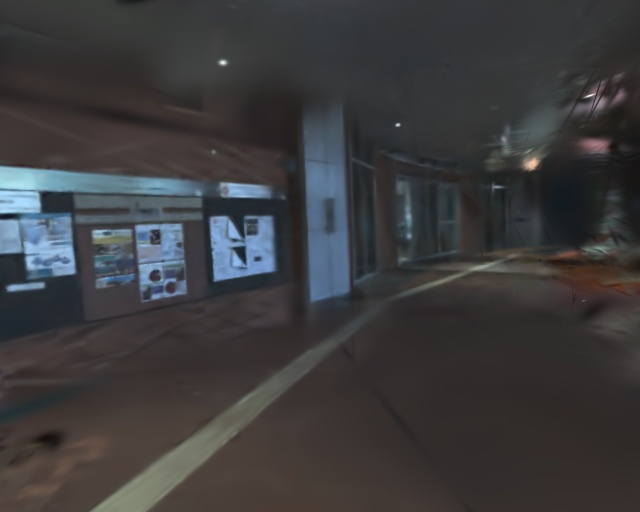
\includegraphics[width=0.30\textwidth]{../../../images/self_compare/ours/train_0784/times_0000.jpg} &
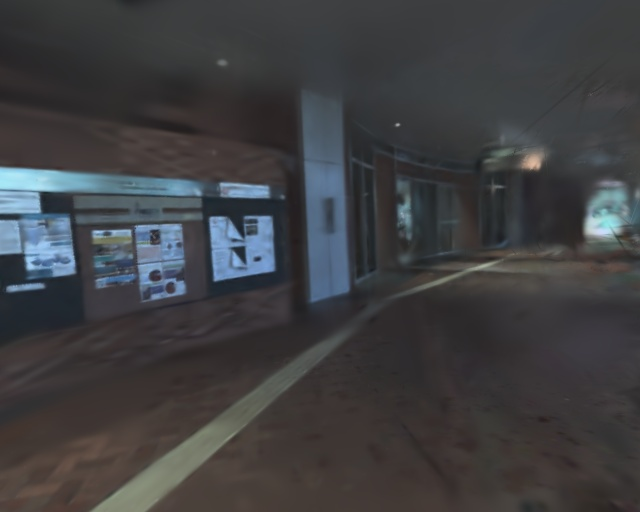
\includegraphics[width=0.30\textwidth]{../../../images/self_compare/ours/train_0784/times_0004.jpg} &
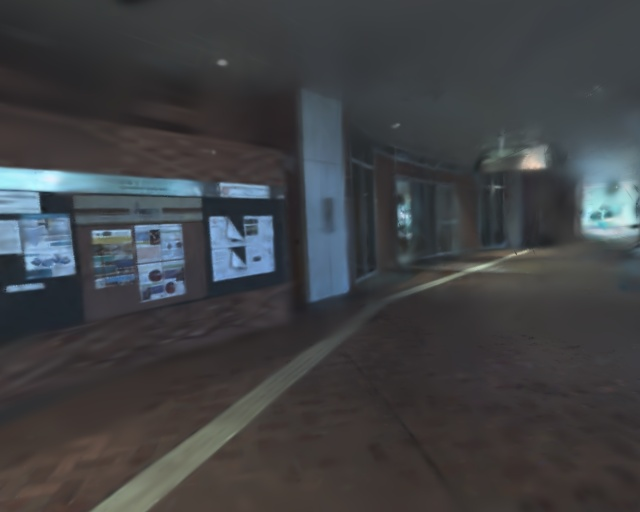
\includegraphics[width=0.30\textwidth]{../../../images/self_compare/ours/train_0784/times_0008.jpg} \\
\end{tabular}
\caption{Visualization results of the feedforward regressor ablation (II). The figure shows the comparison results of representative frames \texttt{train\_0609} and \texttt{train\_0784} under different numbers of local optimization steps. Consistent with Fig.~\ref{fig:ablation_visual_1}, this figure further illustrates the impact of feedforward initialization on subsequent early convergence.}
\label{fig:ablation_visual_2}
\end{figure*}

% \clearpage
% \bibliographystyle{IEEEtran}
% \bibliography{references}
% \clearpage

\end{document}
